\documentclass[c, 9pt, pdftex, xcolor=table]{beamer}
%\usetheme{CEA}
\usepackage{etex}
\usepackage{tabularx}
\usepackage{multirow}
\usepackage{gensymb}
\usepackage[utf8]{inputenc}
%\usepackage[french]{babel}
\usepackage[english]{babel}
%\usepackage{bibentry}
%\nobibliography*
\usepackage[style=alphabetic,citestyle=alphabetic, sorting=nty, backend=bibtex]{biblatex}
\bibliography{../all_my_bib}
\usepackage{listings}
\usepackage{sty/lstlangarm}
%\usepackage{subfig}
\usepackage{verbatim}
\usepackage{sty/stylebeamerCEA}
\usepackage{amsmath}
\usepackage{amssymb}
\usepackage{amsfonts}
\usepackage{amsthm}
\usepackage{siunitx}
\usepackage[table]{xcolor}
\usepackage{graphicx}
\usepackage{array}
\usepackage{subfigure}
%\usepackage{pgfgantt}
\usepackage[normalem]{ulem}
\usepackage[rightcaption]{sidecap}
%\usepackage[export]{adjustbox}
\setbeamertemplate{bibliography item}{\insertbiblabel}
% Permet d'afficher le bandeau CONFIDENTIEL CESTI
\def\bandeauconf#1{
    \textcolor{#1}{
        \renewcommand{\arraystretch}{1.6}
        \begin{tabularx}{\linewidth}{!{\vrule width 1pt}@{}XcX!{\vrule width 1pt}}
        \noalign{\hrule height 1pt}
        &  \textbf{Diffusion restreinte CESTI} & \\
            \noalign{\hrule height 1pt}
        \end{tabularx}
    }
}




%\usepackage{movie15}
\definecolor{grey}{rgb}{0.7,0.7,0.7}
\definecolor{gg}{rgb}{0.85,0.85,0.85}
\definecolor{bb}{rgb}{0.4,0.4,0.4}
%Define colors
\definecolor{blue2}{rgb}{0.3,0.7,1}
\definecolor{blue3}{rgb}{0.4,0.75,1}
\definecolor{blue4}{rgb}{0.55,0.8,1}
\definecolor{blue5}{rgb}{0.7,0.85,1}

%define colors by uses
\definecolor{simcolor}{cmyk}{0.683, 0.482, 0, 0.145} % couleur du simulateur
\definecolor{modcolor}{cmyk}{0.119, 0.547, 0, 0.376} % couleur du modele
\definecolor{gencolor}{cmyk}{0, 0.75, 1, 0.2} % couleur du generateur
\definecolor{filecolor}{cmyk}{0, 0.109, 0.271, 0.031} % couleur des entrees/sorties
\definecolor{gramcolor}{cmyk}{0, 0.4, 1, 0} % couleur du module de grammaire
\definecolor{chipcolor}{cmyk}{0, 0.153, 1, 0} % couleur de la chip d'une càp
\definecolor{attackcolor}{cmyk}{0, 0.2, 1, 0} % couleur des attaques

\definecolor{cpucolor}{cmyk}{0,0.492,0.41,0.522} % couleur du processeur
\definecolor{cocolor}{cmyk}{0.5,1,0,0.2} % couleur des coprocesseurs
\definecolor{memcolor}{cmyk}{0.742,0,0.05,0.529} % couleur de la mémoire
\definecolor{buscolor}{cmyk}{0.555,0,0.486,0.427} % couleur du bus de données
\definecolor{circolor}{cmyk}{0,0,0,0.4} % couleur du fond de circuit

\definecolor{trigcolorleft}{HTML}{7ACC29}
\definecolor{trigcolorright}{HTML}{19D1FF}
\definecolor{trigcolorbottom}{HTML}{336680}

\usepackage{tikz}
%\usepackage{pgfgantt}
\usetikzlibrary{mindmap,backgrounds}
\usetikzlibrary{shapes}
\usetikzlibrary{shapes.symbols}
\usetikzlibrary{decorations.pathreplacing}
\usetikzlibrary{decorations.markings}
\usetikzlibrary{arrows}
\usetikzlibrary{patterns}
\usetikzlibrary{calc}
\usetikzlibrary{positioning}
%\usetikzlibrary{chains,positioning,shapes.symbols,fadings,shadows, backgrounds}
\usetikzlibrary{decorations.pathmorphing}
\usetikzlibrary{shapes.callouts}
%\usetikzlibrary{shapes.arrows, shadings}
\usetikzlibrary{decorations.text}
\usetikzlibrary{matrix}
\usetikzlibrary{shapes}
\usetikzlibrary{shapes.symbols}
\usetikzlibrary{decorations.pathreplacing}


% attaques
\def\attaqueasma{\only<1,2,3>{\#00}\only<4>{\colorbox{attackcolor}{\#04}}}
\def\attaqueasmb{\only<1,2,4>{\#04}\only<3>{\colorbox{attackcolor}{\#ff}}}
\def\attaqueasmc{\only<1,3,4>{\textcolor{green!40!black}{JNC} \textcolor{blue}{DO}}\only<2>{\colorbox{attackcolor}{NOP NOP}}}
\def\attaqueca{\only<1,2,3>{0}\only<4>{\colorbox{attackcolor}{4}}}
\def\attaquecb{\only<1,2,4>{4}\only<3>{\colorbox{attackcolor}{-1}}}
\def\attaquecca{\only<1,3,4>{\itshape\color{purple!40!black}// main loop}
\only<2>{\colorbox{attackcolor}{goto ATTACK;}}}
\def\attaqueccb{\only<1,3,4>{\itshape\color{purple!40!black}// The
comparison is successful}
\only<2>{\colorbox{attackcolor}{ATTACK:}}}

% my new commands

%
\newcommand{\sensVar}{z}
\newcommand{\sensRandVar}{Z}
\newcommand{\sensVarSet}{\mathcal{Z}}
\newcommand{\plaintext}{p}
\newcommand{\randPlaintext}{P}
\newcommand{\plaintextSet}{\mathcal{P}}
\newcommand{\targetFunction}{e}


\newcommand{\key}{k}
\newcommand{\randKey}{K}
\newcommand{\keyTest}{k^{\star}}
\newcommand{\keySet}{\mathcal{K}}
\newcommand{\esper}{\mathbb{E}}
\newcommand{\var}{\mathrm{Var}}
\newcommand{\SNR}{\mathrm{SNR}}

\newcommand{\numTraces}[1][z]{N_{#1}}
\newcommand{\numTracesAttack}{N_a}
\newcommand{\sss}[2][z]{\textbf{x}^{#1}_{#2}} % $\sss{i}$ or $\sss[k]{i}$
\newcommand{\sssTest}[2][z]{\textbf{y}^{#1}_{#2}} % $\sssTest{i}$ or $\sssTest[k]{i}$
\newcommand{\SSS}[1][z]{\textbf{X}^{#1}}
\newcommand{\sssSet}{\mathcal{X}}
\newcommand{\SSSTest}[1][z]{\textbf{Y}_{#1}}
\newcommand{\featureSpace}{\mathcal{F}}

\newcommand{\extractor}[2][]{\varepsilon_{#1}(#2)}
\newcommand{\extract}{\varepsilon}
\newcommand{\bestExtractor}{\varepsilon^\star}

\newcommand{\AAlpha}{\boldsymbol\alpha}
\newcommand{\BBeta}{\boldsymbol\beta}
\newcommand{\mumumu}{\boldsymbol\mu}
\newcommand{\mmm}{\textbf{m}}
\newcommand{\mmmX}{\overline{\textbf{x}}}
\newcommand{\mmmXclass}[1][z]{\overline{\textbf{x}}^{#1}}
\newcommand{\mmmY}{\overline{\textbf{y}}}
%\newcommand{\mmmX}[1][z]{{\bf \meanEst{{\textnormal{$(#1)$}}}}}
%\newcommand{\mmmY}[1][z]{{\bf \meanEst{{\textnormal{$(#1)$}}}}}

\newcommand{\MMM}{\textbf{M}}
\newcommand{\MMMclass}[1][z]{\textbf{M}_{#1}}
\newcommand{\MMMT}{\textbf{M}_{\textbf{T}}}
\newcommand{\NNN}{\textbf{N}}
\newcommand{\III}{\textbf{I}}

\newcommand{\mmmXtot}{{\overline{\bf \meanEst{}}}}

\newcommand{\meanNoise}{{\bf \mu}}
\newcommand{\meanEst}[1]{\mathrm{\bf m}_1 #1 }
\newcommand{\varEst}[1]{\mathrm{m}_2(#1)}
\newcommand{\mean}[2][]{\Bbb{E}_{#1}\left(#2\right)}


\newcommand{\xxx}{\textbf{x}}
\newcommand{\XXX}{\textbf{X}}
\newcommand{\yyy}{\textbf{y}}
\newcommand{\YYY}{\textbf{Y}}
\newcommand{\measuresMatrix}{\textbf{M}}
\newcommand{\projectingMatrix}{\textbf{A}}
\newcommand{\info}[1][z]{\boldsymbol{\varphi}({#1})}
\newcommand{\BBB}{\textbf{B}}
\newcommand{\zero}{\mathbf{0}}
\newcommand{\traceLength}{D}
\newcommand{\newTraceLength}{C}

\newcommand{\numPoI}{\# PoI}

\newcommand{\covmat}{\textbf{S}}


\newcommand{\succRate}{\mathrm{SR}}
\newcommand{\memComplexity}{m}
\newcommand{\guessingVector}{\mathrm{\textbf{g}}}
\newcommand{\adversary}{\mathcal{A}}
\newcommand{\attackAlgorithm}{\mathrm{A}}
\newcommand{\guessingEntropy}{\mathrm{GE}}
\newcommand{\threshold}{\beta}


\newcommand{\vectorContribution}[1][k]{\mathrm{\textbf{ELV}}(#1)}
\newcommand{\varianceInPoints}[2][n]{\mathrm{H}_{#1}(#2)}
\newcommand{\coupleSet}{\mathbb{J}}

\newcommand{\prob}{\mathrm{Pr}}

\newcommand{\SW}{\textbf{S}_{\textbf{W}}}
\newcommand{\SB}{\textbf{S}_{\textbf{B}}}
\newcommand{\ST}{\textbf{S}_{\textbf{T}}}

\newcommand{\vvv}{\textbf{v}}

\newcommand{\EGV}[1]{\mathrm{EGV(#1)}}
\newcommand{\ELV}{\mathrm{ELV}}

\newcommand{\nununu}{\boldsymbol{\nu}}
\newcommand{\NPoI}{N}



%%%%%


\def\firstcircle{(0,0) circle (2.4cm)}

\def\secondcircle{(45:1.8cm) circle (2.4cm)}
\def\thirdcircle{(0:2.4cm) circle (2.4cm)}

\graphicspath{{figs/}}

% itemizecommands
\def\itemyes{\includegraphics[width=0.4cm]{../img/yes}}
\def\itemno{\includegraphics[width=0.4cm]{../img/no}}

% backup commands
\newcommand{\backupbegin}{
   \newcounter{framenumberappendix}
   \setcounter{framenumberappendix}{\value{framenumber}}
}
\newcommand{\backupend}{
   \addtocounter{framenumberappendix}{-\value{framenumber}}
   \addtocounter{framenumber}{\value{framenumberappendix}} 
}

%%%% CONFIGURATION PAQUETAGES %%%%

%% Listings
\lstdefinestyle{customc}{
  belowcaptionskip=1\baselineskip,
  breaklines=true,
  frame=L,
  xleftmargin=\parindent,
  language=C,
  showstringspaces=false,
  basicstyle=\scriptsize\ttfamily,
  keywordstyle=\bfseries\color{green!40!black},
  commentstyle=\itshape\color{purple!40!black},
  identifierstyle=\color{blue},
  stringstyle=\color{orange},
}

\lstdefinestyle{customasm}{
  belowcaptionskip=1\baselineskip,
  frame=L,
  xleftmargin=\parindent,
  language=[x86masm]Assembler,
  basicstyle=\tiny\ttfamily,
  commentstyle=\itshape\color{purple!40!black},
  morecomment=[l]{//},
  morekeywords={SUBB},
}

\lstset{ numbers=left, tabsize=3, frame=single, numberstyle=\ttfamily,
basicstyle=\footnotesize, style=customc,
           captionpos=b, % sets the caption position to bottom
               extendedchars=false, % for babel compatibility
}

\setbeamertemplate{section in toc shaded}[default][50]
\AtBeginSection[]
{
  \frame<handout:0>
  {
    \frametitle{Contents}
    \tableofcontents[sectionstyle=show/shaded,
    subsectionstyle=show/show/shaded, subsubsectionstyle=show/show/show/shaded]
  }
}

\def\etal{\textit{et al.} }
\newcommand {\ie}{{\em i.e.} }
\def\eg{\textit{e.g.} }
\def\via{\textit{via} }
 
%define colors by uses
\definecolor{standardcolor}{rgb}{1.0,1.0,1.0}
\definecolor{simcolor}{cmyk}{0.683, 0.482, 0, 0.145} % couleur du simulateur
\definecolor{modcolor}{cmyk}{0.119, 0.547, 0, 0.376} % couleur du modele
\definecolor{gencolor}{cmyk}{0, 0.75, 1, 0.2} % couleur du generateur
\definecolor{filecolor}{cmyk}{0, 0.109, 0.271, 0.031} % couleur des entrees/sorties
\definecolor{gramcolor}{cmyk}{0, 0.4, 1, 0} % couleur du module de grammaire
\definecolor{chipcolor}{cmyk}{0, 0.153, 1, 0} % couleur de la chip d'une càp
\definecolor{attackcolor}{cmyk}{0, 0.2, 1, 0} % couleur des attaques

\definecolor{cpucolor}{cmyk}{0,0.492,0.41,0.522} % couleur du processeur
\definecolor{cocolor}{cmyk}{0.5,1,0,0.2} % couleur des coprocesseurs
\definecolor{memcolor}{cmyk}{0.742,0,0.05,0.529} % couleur de la mémoire
\definecolor{buscolor}{cmyk}{0.555,0,0.486,0.427} % couleur du bus de données
\definecolor{circolor}{cmyk}{0,0,0,0.4} % couleur du fond de circuit

\newsavebox\chip
\sbox{\chip}{

\begin{tikzpicture}[remember picture,
scale=0.07,
% define styles here
chiplayout/.style={rectangle, draw, fill=chipcolor, rounded corners}
]
\draw[chiplayout] (0, 0) rectangle (9,8);
\draw (3, 0) -- (3, 8);
\draw (3, 2) -- (0, 2);
\draw (3, 4) -- (0, 4);
\draw (3, 6) -- (0, 6);

\draw (6, 0) -- (6, 6);
\draw (6, 2) -- (9, 2);
\draw (6, 4) -- (9, 4);
\draw (6, 6) -- (9, 6);
\end{tikzpicture}
}

\tikzstyle{block} = [rectangle, draw, text width=6em, text centered, rounded corners, minimum height=4em]

\tikzset{middlearrow/.style={
        decoration={markings,
            mark= at position 0.5 with {\arrow{#1}} ,
        },
        postaction={decorate}
    }
}

% tikz block styles
\tikzstyle{decision} =  [diamond, draw, fill=blue!20,
text width=5.5em, text badly centered, node distance=3.2cm, inner
sep=0pt]
\tikzstyle{block} = [rectangle, draw, fill=blue!20,
text width=7.0em, text centered, node distance=3.2cm, rounded corners, minimum height=3em]
\tikzstyle{line} = [draw, -latex']
\tikzstyle{cloud} = [draw, ellipse, fill=red!20, node distance=3cm, 
minimum height=2em]




\title[]{Feature Extraction for Side-Channel Attacks}
%\subtitle{\emph{Analysis and Research of Points of Interest in the Context of Side-Channel Attacks on Smart Card}}

\author{Eleonora Cagli}


\date{05/12/2018, Paris}

\colorlet{codecolor}{standardcolor}
\colorlet{objcolor}{standardcolor}
\colorlet{modelecolor}{standardcolor}
\colorlet{outilscolor}{standardcolor}
\colorlet{mutantscolor}{standardcolor}
\colorlet{oraclecolor}{standardcolor}
\colorlet{attaquescolor}{standardcolor}


% Repartir du pb:

\begin{document}
%\inserttitlepage
% Titleframe
\setbeamertemplate{background
canvas}{\includegraphics[width=\paperwidth,height=\paperheight]{img-templates/fondceatech}}
\begin{frame}[plain]
	\small
  	\vspace{0.5cm}
	\begin{columns}

	\begin{column}{.36\textwidth}
		\hspace{0.5cm}
	\end{column}

	\begin{column}{.64\textwidth}
		\centering
  		\titlepage
  		\vspace{0.5cm}
		
  		\vspace{0.5cm}
	\end{column}

\end{columns}



\begin{columns}
\begin{column}{\textwidth}
\hfill \emph{PhD Supervisor :} Emmanuel Prouff\\
\hfill \footnotesize{(Safran Identity \& Security)}\\
\hfill \small{\emph{CEA Supervisor :} C\'ecile Dumas\textcolor{white}{}} \\
\hfill \footnotesize{(CEA-Leti Grenoble)}
\end{column}
\end{columns}


\end{frame}

\setbeamertemplate{background canvas}{}



\section{Context and State of the Art}

\begin{frame}
\vspace{-15pt}
\frametitle{Context}
\begin{block}{Side-Channel Attacks (SCAs)}
\begin{itemize}
\item Target: a physical implementations of cryptographic primitives 
\item Means: observable physical variations (timing information, power consumption, electromagnetic irradiation, etc.)
\item Goal: retrieve secret data (ex: cryptographic key)
\end{itemize}
\end{block}

\begin{block}{Notations}
\begin{itemize}
\item Side-channel traces: realizations of a random variable $\XXX \in \mathbb{R}^D$  (column vector)
\item Target: a \emph{sensitive} variable $Z = f(P,K)\in\sensVarSet$ 
\end{itemize}
\end{block}
\vspace{-5pt}
\begin{block}{Profiling attack scenario}
Exploits labelled traces $(\sss[z_i]{i})_{i=1}^N$ to characterize the signals in function of $z_i$.\\
\emph{"a trace $\sss[z]{}$ belongs to the class $z$"}
\end{block}
%\begin{small}
%\emph{Example: Gaussian Template Attack} 
%\begin{itemize}
%\item Profiling phase: estimate the parameters $\{(\mumumu_z,\Sigma_z)\}_{z\in\sensVarSet}$ of multivariate Gaussian distributions
%\item Attack phase: rank key hypothesis through maximum likelihood
%\end{itemize}
%\end{small}



\end{frame}




%\begin{frame}
%\vspace{-5pt}
%\frametitle{Points of Interest}
%\vspace{-10pt}
%
%\begin{block}{Problem}
%Highly multi-dimensional side-channel traces (algorithm, instruments sampling rate, etc.)\\
%$\longrightarrow$ affects attack complexity
%\end{block}
%
%\includegraphics[width = 0.4\textwidth]{figures/power_trace.pdf}
%\only<2>{
%\includegraphics[width = 0.4\textwidth]{figures/SNR_trace.pdf}
%}
%
%\begin{block}{Which part characterize?}
%Only (relatively) few points depend on the target: the \emph{Points of Interest (PoIs)}
%\end{block}
%
%\pause
%\begin{block}{How to find them?}
%A first answer: statistical tests.\\
%For example estimating the SNR:
%\begin{equation}
%\SNR = \frac{\var(\esper[\XXX\vline Z])}{\esper[\var(\XXX\vline Z)]}
%\end{equation}
%\end{block}
%
%
%\end{frame}




\begin{frame}
\frametitle{Dimensionality Reduction}

\begin{block}{Problem}
Highly multi-dimensional side-channel traces (algorithm, sampling rate, etc.)\\
$\longrightarrow$ affect attack complexity
\end{block}

\begin{block}{Goal}
Perform a preprocessing via an opportune \emph{extractor} $\extract:\mathbb{R}^D\rightarrow \mathbb{R}^C$ in order to:
\begin{itemize}
\item Reduce memory and time complexity (ameliorate the attacks efficiency in terms of required samples)
\item Enhance contribution of the Points of Interest (PoI, those that depend on the target) to concentrate information over few points (ameliorate the attacks efficiency in terms of required traces)
\end{itemize}
\end{block}

%\begin{block}{Extractor}
%\begin{equation}
%\extract:\mathbb{R}^D\rightarrow \mathbb{R}^C
%\end{equation}
%\end{block}


\end{frame}

\begin{frame}
\frametitle{Literature}
Two typologies of extractors in literature
\begin{block}{Selecting Extractors}
$\extract$ performs a sub-sampling
\begin{itemize}
\item Sum of Differences (SOD) \cite{Chari2003}
\item Signal-to-Noise Ratio (SNR) \cite{mangard2008power}
\item Sum of Squared $t$-differences (SOST), $t$-test, $F$-test,... \cite{gierlichs2006templates,bar2010improved,choudary2014efficient}
\end{itemize}
\end{block}

\begin{block}{Projecting Extractors}
$\extract(\sss[]{}) = A\sss[]{} \mbox{ with } A \in M_{\mathbb{R}}(\newTraceLength, \traceLength)$
\begin{itemize}
\item Principal Component Analysis (PCA) \cite{TAprincipal,Batina2012}
\item Linear Discriminant Analysis (LDA) \cite{Standaert2008,lessIsMore}
\end{itemize}
\end{block}

\end{frame}


\section{State of the Art, Objectives, Contributions}

\begin{frame}
\frametitle{Notations}

\end{frame}

\begin{frame}
\frametitle{Template Attack} 
% aprendo des volets per ogni passaggio con riferimenti allo stato dell'arte:
% templates : likelihood vs MAP ,  cov mats vs pooled , linear regression or not
% dimensionality reduction : feature selection, feature extraction, masking : masques connus vs unconnus
% misalignment : re-alignement

\end{frame}

\begin{frame}
\frametitle{Contributions}
\begin{block}{Objective}

\end{block}
% le même dessin que template attack avec le point où on en est du processus et la téchnique étudiée
\end{frame}
%
%\begin{frame}
%\frametitle{Projecting Extractors: PCA and LDA}
%\begin{figure}
%\centering{
%\resizebox{11cm}{!}
%{
%\begin{tikzpicture}[remember picture,
%    scale=0.50,
%    % Define styles here
%    every node/.style={transform shape}
%    block/.style={
%        rectangle,
%        draw,
%        text centered,
%        rounded corners
%        },
%    data/.style={
%        trapezium,
%        trapezium left angle=60,
%        trapezium right angle=120,
%        draw
%        },
%    component/.style={
%        circle,
%        draw
%        },
%    output/.style={
%        tape,
%        tape bend top=none,
%        draw
%        },
%    edge/.style={
%        ->,
%        >=stealth,
%        thick
%        }
%    ]
%
%    % Place nodes
%    \node[inner sep=0pt] (genericTrace) at (0,-0)
%    {\includegraphics[width=0.8\textwidth]{figures/genericTrace.pdf} };
%    \node [above=0.1cm of genericTrace] {Rough Trace};
%    \node [block, below left=0.8cm of genericTrace] (PCA) {\begin{Large}PCA\end{Large}};
%    \node [block, below right=0.8cm of genericTrace] (LDA) {\begin{Large}LDA\end{Large}};
%    \node [below=1.5cm of genericTrace](puntini) {\begin{Large}$\dots$\end{Large}};
%    \node [component, left=0.5cm of puntini](PC2) {\begin{Large}$\AAlpha_2$\end{Large}};
%    \node [component, left=0.5cm of PC2](PC1) {\begin{Large}$\AAlpha_1$\end{Large}};
%    \node [component, right=0.25cm of puntini](PCC) {\begin{Large}$\AAlpha_C$\end{Large}};
%   \node [right=0.25cm of PCC](puntini2) {\begin{Large}$\dots$\end{Large}};
%    \node [component, right=0.15cm of puntini2](PCr) {\begin{Large}$\AAlpha_r$\end{Large}};
%    %\draw[thick, black,decorate,decoration={brace,amplitude=10pt}](PC1.north) -- (PCr.north);
%    \draw(PC1.north)  to [bend left=15] (PCr.north);
%    
%    
%    \draw[->, shorten >=20pt] (PCA.north) node[above=0.4cm] {Principal Components (PCs)} to [bend left] (PC2.north) ;
%     \draw[->,shorten >=25pt] (LDA.north)  node[above=0.35cm] {Discriminant Components (DCs)} to [bend right] (puntini2.north);
%     
%    \only<2>{ 
%    \node [data, below=1cm of puntini](formula1) {\begin{Large}$\sum_{j=1}^D\AAlpha_1[j]\textbf{x}[j]$\end{Large}};
%    \node [left=0.5cm of formula1] {Linear Combination / Projection};
%    \node [below=0.5cm of formula1] (compressed1)
%    	{\includegraphics[width=0.5\textwidth]{figures/compressed1.pdf} }; 
%    	\node[right=0.1cm of compressed1]{Reduced Trace}; 
%	\draw[-, red, thick, shorten >=6pt, shorten <=-6pt](genericTrace.south) to (PC1.north);
%	\draw[-, red, thick, shorten >=6pt, shorten <= 6pt](PC1.south) to (formula1.north);
%	\draw[-, red, thick, shorten <= 2pt, shorten >=-5pt](formula1.south) to (compressed1.north);
%}
%    
%        \only<3>{ 
%        \node [data, below=1cm of puntini](formula2) {\begin{Large}$\sum_{j=1}^D\AAlpha_2[j]\textbf{x}				[j]$\end{Large}};
%    \node [left=0.5cm of formula2] {Linear Combination / Projection};
%    \node [below=0.5cm of formula2] (compressed2)
%    	{\includegraphics[width=0.5\textwidth]{figures/compressed2.pdf} };  
%    	\node[right=0.1cm of compressed2]{Reduced Trace};
%	\draw[-, red, thick, shorten >=6pt, shorten <=-6pt](genericTrace.south) to (PC2.north);
%	\draw[-, red, thick, shorten >=6pt, shorten <= 6pt](PC2.south) to (formula1.north);
%	\draw[-, red, thick, shorten <= 2pt, shorten >=-5pt](formula2.south) to (compressed2.north);
%}
%
% \uncover<4>{ 
%        \node [data, below=1cm of puntini](formulaC) {\begin{Large}$\sum_{j=1}^D\AAlpha_C[j]\textbf{x}				[j]$\end{Large}};
%    \node [left=0.5cm of formulaC] {Linear Combination / Projection};
%    \node [below=0.5cm of formulaC] (compressedC)
%    	{\includegraphics[width=0.5\textwidth]{figures/compressedAll.pdf} }; 
%    \node[right=0.1cm of compressedC]{Reduced Trace};
%	\draw[-, red, thick, shorten >=6pt, shorten <=-6pt](genericTrace.south) to (PCC.north);
%	\draw[-, red, thick, shorten >=6pt, shorten <= 6pt](PCC.south) to (formulaC.north);
%	\draw[-, red, thick, shorten <= 2pt, shorten >=-5pt](formulaC.south) to (compressedC.north);
%}
%    
%     
%     
%
%\end{tikzpicture}
%}
%}
%
%\end{figure}
%\end{frame}



\begin{frame}
\frametitle{PCA and LDA}
\only<1>{
\vspace{-50pt}
\begin{block}{Standard PCA}
\begin{itemize}
\item maximizing data variance
\item not exploiting sensitive variable knowledge
\end{itemize}
\end{block}
\vfill
}
\only<2->{
\begin{block}{Class-oriented PCA}
\begin{itemize}
\item\only<2->{eigenvector research}
\item \only<2->{maximizing inter-class variance}
\item \only<3->{not minimizing the intra-class variance}
\item \only<4->{easily and accurately computable (no matrix inversions)}
\item \only<5->{\textcolor{red}{components selection issue} (disagreement between theory and experience)$\longrightarrow $ ELV selection tool [CARDIS 2015]}
\end{itemize}
\end{block}
}
\only<2-5>{
\begin{block}{LDA}
\begin{itemize}
\item\only<2-5>{eigenvector research}
\item \only<2-5>{maximizing inter-class variance while minimizing intra-class variance (no loss of information under some leakage model \cite{lessIsMore})}
\item \only<4-5> {not easily computable (asking for a matrix inversion)}
\end{itemize}
\end{block}
}



\end{frame}

\begin{frame}
\frametitle{Overview of experimental results of the ELV selection tool}
\begin{block}{Overview of experimental results of the ELV selection tool}
\begin{itemize}
\item large profiling set: PCA performances close to the LDA's if equipped with ELV (and less expensive)
\item small profiling set: LDA efficiency decreases faster than (PCA $+$ ELV)'s \item too small profiling set: LDA unavailable. PCA$+$ELV still efficient
\end{itemize}

\end{block}
\end{frame}

\begin{frame}
\frametitle{Contents}
\begin{itemize}
\item \textcolor{grey}{Introduction to LDA: as a classifier, and as a feature extractor}
\item \important{Introduction to masking countermeasure and Kernel Discriminant Analysis as a feature extractor}
\item Convolutional Neural Networks and Data Augmentation to attack jitter-based countermeasure
\end{itemize}
\end{frame}

%\subsubsection{Components Selection Issue}
%
%\begin{frame} \frametitle{The Problem of Selecting PCA Components}
%
%% state of the art
%% first and sixth PC DPA contest
%\begin{columns}
%\begin{column}{0.1\textwidth}
%\includegraphics[width = \textwidth]{figures/questionmark.jpg} 
%\end{column}
%\begin{column}{0.7\textwidth}
%\begin{block}{}
%{\em How many} PCs and {\em which ones} are sufficient/necessary to reduce the traces size without losing important discriminant information?
%\end{block}
%\end{column}
%\end{columns}
%\vspace{-7pt}
%\begin{block}{Experimental Observation}
%\cite{Batina2012,specht}: the first components sometimes contain no sensitive information; it is worth discarding them.
%\end{block}
%\begin{figure}
%\includegraphics[width=.45\textwidth]{figures/DPAcontestPC1_new.pdf} 
%\includegraphics[width=.45\textwidth]{figures/DPAcontestPC6_new.pdf} 
%\caption{First and sixth PCs in DPA contest v4  \cite{DPAcontest} trace set}\label{fig:DPAcontest}
%\end{figure}
%
%
%
%
%
%\end{frame}
%
%
%\begin{frame} \frametitle{The Problem of Selecting PCA Components - EGV, IPR}
%\begin{block}{Explained Global Variance (EGV)}
%$\EGV{\AAlpha_i} = \frac{\lambda_i}{\sum_{k=1}^r \lambda_k}$\\
%\cite{choudaryefficient} : 
%\begin{itemize}
%\item fix a threshold $\beta$
%\item choose the first $C$ components, where $C$ is the minimum integer such that
%\begin{equation*}
%\EGV{\AAlpha_1}+ \EGV{\AAlpha_2}+\dots + \EGV{\AAlpha_C} \geq \beta
%\end{equation*}
%\end{itemize}
%\end{block}
%%\begin{block}{Assumption}
%%Dealing with secured devices, the leaking side-channel information is localised in few points of the acquired trace.
%%\end{block}
%
%\begin{block}{Inverse Participation Ratio (IPR)}
%\cite{SCAclassProbl}: 
%\begin{equation*}
%\mathrm{IPR}(\AAlpha_i) = \sum_{j=1}^\traceLength \AAlpha_i[j]^4 \mbox{ \em (localization score)}
%\end{equation*}
%\end{block}
%\end{frame}


%\begin{frame} \frametitle{The Component Selection Issue}
%
%\begin{columns}
%\begin{column}{0.1\textwidth}
%\includegraphics[width = \textwidth]{figures/questionmark.jpg} 
%\end{column}
%\begin{column}{0.7\textwidth}
%\begin{block}{}
%{\em How many} PCs and {\em which ones} are sufficient/necessary to reduce the traces size without losing important discriminant information? 
%\end{block}
%\end{column}
%\end{columns}
% \only<1>{
% \begin{block}{Theoretically}
%Higher eigenvalues $\longrightarrow$ higher information.
%\end{block}
%\begin{block}{Experimental Observation}
%\cite{Batina2012,specht}: the first components sometimes contain no sensitive information; it is worth discarding them.
%\end{block}
%
%\begin{figure}
%\includegraphics[width=.25\textwidth]{figures/DPAcontestPC1_new.pdf} 
%\includegraphics[width=.25\textwidth]{figures/DPAcontestPC6_new.pdf} 
%\vspace{-10pt}
%\caption{First and sixth PCs in DPA contest v4  \cite{DPAcontest} trace set}\label{fig:DPAcontest}
%\end{figure}
%}
%\only<2>{
%\vspace{40pt}
%\begin{small}
%\begin{table}
%\begin{tabular}{|c|c|c|c|}
%\hline
%& EGV \cite{choudaryefficient} & IPR \cite{SCAclassProbl}& \uncover<2->{\textbf{ELV} \cite{Cagli2016}} \\
%\hline
%eigenvalue $\lambda_i$ &\includegraphics[scale=0.01]{figures/yes.png}  & \includegraphics[scale=0.01]{figures/no.png} &\uncover<2->{\includegraphics[scale=0.015]{figures/yes.png}}\\
%\hline
%form of $\AAlpha_i$ &\includegraphics[scale=0.01]{figures/no.png}  & \includegraphics[scale=0.01]{figures/yes.png}&\uncover<2->{\includegraphics[scale=0.015]{figures/yes.png}} \\
%\hline
%\end{tabular}
%\end{table}
%\end{small}
%
%\includegraphics[scale=0.3]{figures/citazione1.jpg} 
%}
%\uncover<2->{
%\begin{block}{Explained Local Variance}
%$\mathrm{ELV}(\AAlpha_i,j) = \frac{\lambda_i \AAlpha_i[j]^2}{\sum_{k=1}^r\lambda_k} = \mathrm{EGV}(\AAlpha_i) \AAlpha_i[j]^2$  \\
%%($\sum_{j=1}^D \mathrm{ELV}(\AAlpha_i,j) = \EGV{\AAlpha_i}$)
%\end{block}
%}
%\uncover<3->{\begin{block}{Use of the ELV}
%\begin{itemize}
%\item Sort in decreasing order the maximal ELV provided by each component $\{\max_{j=1,\dots,D}\ELV(\AAlpha_i,j)\}_{i}$ and select the $C$ first components.
%\item Select \textbf{couples} $(\AAlpha_i, j)$ in decreasing order wrt to $\ELV(\AAlpha_i, j)$ until $\ELV(\AAlpha_{i_1}, j_1)+ \ELV(\AAlpha_{i_2}, j_2)+\dots +\ELV(\AAlpha_{i_M}, j_M)\geq \beta$
%\end{itemize}
%\end{block}}
%\end{frame}

%\begin{frame} \frametitle{The ELV Selection (2)}
%\vspace*{-0.5cm}
%\uncover<1->{
%\begin{block}{Definition}
%$\mathrm{ELV}(\AAlpha_i,j) = \frac{\lambda_i \AAlpha_i[j]^2}{\sum_{k=1}^r\lambda_k} = \mathrm{EGV}(\AAlpha_i) \AAlpha_i[j]^2$  \\
%\uncover<2->{Observe that $\sum_{j=1}^D \mathrm{ELV}(\AAlpha_i,j) = \EGV{\AAlpha_i}$}
%\end{block}
%}
%\uncover<3->{
%Perform this sum in a cumulative way, sorting the ELV contributions of the time samples in decreasing order, {\em i. e.} $\mathrm{ELV}(\AAlpha_i,j^i_1)\geq \mathrm{ELV}(\AAlpha_i,j^i_2)\geq \dots \geq \mathrm{ELV}(\AAlpha_i,j^i_\traceLength)$
%
%
%\vspace*{-0.4cm}
%\begin{columns}
%\begin{column}{.5\textwidth}
%\vspace*{10pt}
%\begin{figure}
%\includegraphics[width=\textwidth]{figures/PC1_points.pdf} 
%\end{figure}
%\end{column}
%\begin{column}{.5\textwidth}
%\begin{figure}
%
%\begin{tikzpicture}[remember picture,
%    scale=1,
%    % Define styles here
%    every node/.style={transform shape}
%    block/.style={
%        rectangle,
%        draw,
%        text centered,
%        rounded corners
%        },
%    data/.style={
%        trapezium,
%        trapezium left angle=60,
%        trapezium right angle=120,
%        draw
%        },
%    component/.style={
%        circle,
%        draw
%        },
%    output/.style={
%        tape,
%        tape bend top=none,
%        draw
%        },
%    edge/.style={
%        ->,
%        >=stealth,
%        thick
%        }
%    ]
%
%    \node (only1elv) at (0,0)
%    {\includegraphics[width=\textwidth]{figures/cumulativeELV_only1.pdf} };
%    \node [component, thick, xshift=2.1cm, yshift=0.8cm] (cerchio) {};
%    \node[below left=1cm of cerchio](caption){$\mathrm{EGV}(\AAlpha_1)$};
%    \draw[->] (caption) to (cerchio.south west);
%\end{tikzpicture}
%\end{figure}
%\end{column}
%\end{columns}
%
%
%}
%
%\end{frame}



%\begin{frame}
%\frametitle{The ELV Selection (2)}
%\begin{columns}
%\begin{column}{0.5\textwidth}
%\uncover<1->{
%\only<1>{
%\vspace*{-0.4cm}
%\begin{center}
%\includegraphics[width = \textwidth]{figures/cumulativeELV.pdf}
%\end{center}
%}
%\only<2>{
%\vspace*{-0.4cm}
%\begin{center}
%\includegraphics[width = \textwidth]{figures/cumulativeELVallRectangle.pdf} 
%\end{center}
%}
%
%\only<3->{
%\vspace*{-0.4cm}
%\begin{center}
%\includegraphics[width = \textwidth]{figures/cumulativeELVzoomed.pdf}
%\end{center}
%}
%}
%\uncover<4->{
%\only<1-4>{
%
%\begin{block}{To select $C$ components\hspace{\textwidth}\textcolor{white}{ }}
%Sort in decreasing order the maximal ELV provided by each component $\{\max_{j=1,\dots,D}\ELV(\AAlpha_i,j)\}_{i}$ and select the $C$ first components.
%\end{block}
%}
%\only<5>{
%
%\begin{block}{Fixing a cumulative explained variance threshold $\beta$}
%Select \textbf{couples} $(\AAlpha_i, j)$ in decreasing order wrt to $\ELV(\AAlpha_i, j)$ until $\ELV(\AAlpha_{i_1}, j_1)+ \ELV(\AAlpha_{i_2}, j_2)+\dots +\ELV(\AAlpha_{i_M}, j_M)\geq \beta$.\\
%%\uncover<5>{{\em Components denoising}}
%\end{block}
%}
%}
%
%\end{column}
%
%\begin{column}{0.5\textwidth}
%\only<1-3>{
%\begin{figure}
%\includegraphics[width=0.5\textwidth]{figures/PC1.pdf} 
%\includegraphics[width=0.5\textwidth]{figures/PC4.pdf} \\
%\includegraphics[width=0.5\textwidth]{figures/PC2.pdf} 
%\includegraphics[width=0.5\textwidth]{figures/PC5.pdf} \\
%\includegraphics[width=0.5\textwidth]{figures/PC3.pdf} 
%\includegraphics[width=0.5\textwidth]{figures/PC6.pdf} 
%\caption{\begin{footnotesize}
%The first 6 PCs: 
%$\lambda_1 \approx 3.8 ,\lambda_2 \approx 3.1 , \lambda_3 \approx2.6 ,\lambda_4 \approx 1.0 ,\lambda_5 \approx 0.8 ,\lambda_6 \approx 0.6 $
%\end{footnotesize}}
%
%\end{figure}
%}


%\only<4-5>{
%\begin{figure}
%\onslide<5->{\includegraphics[width=0.5\textwidth]{figures/PC5_denoised.pdf}}\only<4>{\includegraphics[width=0.5\textwidth]{figures/PC5_cerchio.pdf}}\only<5>{\includegraphics[width=0.5\textwidth]{figures/PC5_cerchio_transp.pdf}} \\
%\onslide<5->{\includegraphics[width=0.5\textwidth]{figures/PC4_denoised.pdf}}\only<4>{\includegraphics[width=0.5\textwidth]{figures/PC4_cerchio.pdf}}\only<5>{\includegraphics[width=0.5\textwidth]{figures/PC4_cerchio_transp.pdf}} \\
%\onslide<5->{\includegraphics[width=0.5\textwidth]{figures/PC6_denoised.pdf}}\only<4>{\includegraphics[width=0.5\textwidth]{figures/PC6_cerchio.pdf}}\only<5>{\includegraphics[width=0.5\textwidth]{figures/PC6_cerchio_transp.pdf}} 
%\only<4>{\caption{The 3 components chosen by ELV selection method - $C$ fixed}}
%\only<5>{\caption{Components and time samples chosen by ELV selection method - $\beta$ fixed}}
%\end{figure}
%}


%\only<5>{
%\includegraphics[width=0.31\textwidth]{figures/PC5_cerchio_transp.pdf} 
%\includegraphics[width=0.31\textwidth]{figures/PC4_cerchio_transp.pdf} 
%\includegraphics[width=0.31\textwidth]{figures/PC6_cerchio_transp.pdf} \\
%}
%\uncover<5>{
%
%
%
%\only<3-4>{\caption{Selected components for $C = 3$; \hspace{\textwidth} $\ELV(\AAlpha_5, 2362)\approx 0.41$, $\ELV(\AAlpha_4, 1110)\approx 0.38$, $\ELV(\AAlpha_6, 1118)\approx 0.24$}}
%\only<5>{\caption{Selected and denoised components for $\beta = 0.08$\hspace{\textwidth}\textcolor{white}{$\ELV(\AAlpha_5, 2362)\approx 0.41$, $\ELV(\AAlpha_4, 1110)\approx 0.38$, $\ELV(\AAlpha_6, 1118)\approx 0.24$}}}
%
%\end{column}
%
%\end{columns}
%
%
%\end{frame}

%\subsection{Linear Discriminant Analysis}
%
%
%\subsubsection{The Small Sample Size (SSS) Problem}
%
%\begin{frame} \frametitle{The Small Sample Size (SSS) Problem}
%\begin{block}{The SSS Problem}
%$\SW$ has to be invertible \\
%
%
%Necessary condition: the total number of acquisition used to construct $\SW$ must be higher than $D$
%\end{block}
%
%
%\begin{block}{A Glance to the Pattern Recognition State of the Art}
%Four methods: 
%\begin{itemize}
%\item \cite{eigenfaces}: Fisherface
%\item \cite{Chen2000} : $\SW$ Null Space
%\item \cite{Yu01adirect} : Direct LDA
%\item \cite{huang} : $\ST$ Spanned Space 
%\end{itemize}
%\end{block}
%\end{frame}
%

%\subsection{Experimental Results}
%
%
%
%
%
%\begin{frame}
%\vspace*{-2pt}
%\frametitle{Experimental results (minimizing $N_a$)}
%\vspace{-10pt}
%\begin{figure}[t]
%\includegraphics[width=0.4\textwidth]{figures/Criterion1.pdf}
%\includegraphics[width=0.4\textwidth]{figures/Criterion1Good.pdf}
%\caption{Guessing Entropy as function of the number of attack traces.}
%\end{figure}
%\vspace{-10pt}
%\begin{block}{Observations}
%\begin{itemize}
%\item LDA optimal (but more expensive)
%\item PCA close to LDA if equipped with ELV (and less expensive)
%\end{itemize}
%\end{block}
%
%\end{frame}
%
%\begin{frame}
%\vspace*{-2pt}
%\frametitle{Experimental results (minimizing $N_p$)}
%
%\vspace{-10pt}
%\begin{figure}
%\includegraphics[width=0.4\textwidth]{figures/SSS.pdf}
%\includegraphics[width=0.4\textwidth]{figures/Criterion2notSSS.pdf}
%\caption{Guessing Entropy as function of the number of profiling traces.}
%\end{figure}
%
%\begin{block}{Observations}
%\begin{itemize}
%\item if LDA unavailable: PCA$+$ELV best alternative
%\item if LDA available: its efficiency is affected by the lack of profiling traces, PCA $+$ ELV keeps better
%\end{itemize}
%\end{block}
%
%\end{frame}
%\section{Kernel Discriminant Analysis against Masking}
\subsection{Linear Discriminant Analysis}

%\begin{frame}
%\frametitle{Contents}
%\begin{itemize}
%\item \important{Introduction to LDA: as a classifier, and as a feature extractor}
%\item Introduction to masking countermeasure and Kernel Discriminant Analysis as a feature extractor
%\item Motivations to apply deep learning techniques
%\item Convolutional Neural Networks and Data Augmentation to attack jitter-based countermeasure
%\end{itemize}
%\end{frame}

\begin{frame}{Linear Dimensionality Reduction}
\begin{figure}
\centering{
\resizebox{11cm}{!}
{
\begin{tikzpicture}[remember picture,
    scale=0.50,
    % Define styles here
    every node/.style={transform shape}
    block/.style={
        rectangle,
        draw,
        text centered,
        rounded corners
        },
    data/.style={
        trapezium,
        trapezium left angle=60,
        trapezium right angle=120,
        draw
        },
    component/.style={
        circle,
        draw
        },
    output/.style={
        tape,
        tape bend top=none,
        draw
        },
    edge/.style={
        ->,
        >=stealth,
        thick
        }
    ]

    % Place nodes
    \node[inner sep=0pt] (genericTrace) at (0,-0)
    {\includegraphics[width=0.8\textwidth]{figures/genericTrace.pdf} };
    \node [above=0.1cm of genericTrace] {Rough Trace};
    \node [block, below left=0.8cm of genericTrace] (PCA) {\begin{Large}PCA\end{Large}};
    \node [block, below right=0.8cm of genericTrace] (LDA) {\begin{Large}LDA\end{Large}};
    \node [below=1.5cm of genericTrace](puntini) {\begin{Large}$\dots$\end{Large}};
    \node [component, left=0.5cm of puntini](PC2) {\begin{Large}$\AAlpha_2$\end{Large}};
    \node [component, left=0.5cm of PC2](PC1) {\begin{Large}$\AAlpha_1$\end{Large}};
    \node [component, right=0.25cm of puntini](PCC) {\begin{Large}$\AAlpha_C$\end{Large}};
   \node [right=0.25cm of PCC](puntini2) {\begin{Large}$\dots$\end{Large}};
    \node [component, right=0.15cm of puntini2](PCr) {\begin{Large}$\AAlpha_r$\end{Large}};
    %\draw[thick, black,decorate,decoration={brace,amplitude=10pt}](PC1.north) -- (PCr.north);
    \draw(PC1.north)  to [bend left=15] (PCr.north);
    
    
    \draw[->, shorten >=20pt] (PCA.north) node[above=0.4cm] {Principal Components (PCs)} to [bend left] (PC2.north) ;
     \draw[->,shorten >=25pt] (LDA.north)  node[above=0.35cm] {Discriminant Components (DCs)} to [bend right] (puntini2.north);
     
    \only<2>{ 
    \node [data, below=1cm of puntini](formula1) {\begin{Large}$\sum_{j=1}^D\AAlpha_1[j]\textbf{x}[j]$\end{Large}};
    \node [left=0.5cm of formula1] {Linear Combination / Projection};
    \node [below=0.5cm of formula1] (compressed1)
    	{\includegraphics[width=0.5\textwidth]{figures/compressed1.pdf} }; 
    	\node[right=0.1cm of compressed1]{Reduced Trace}; 
	\draw[-, red, thick, shorten >=6pt, shorten <=-6pt](genericTrace.south) to (PC1.north);
	\draw[-, red, thick, shorten >=6pt, shorten <= 6pt](PC1.south) to (formula1.north);
	\draw[-, red, thick, shorten <= 2pt, shorten >=-5pt](formula1.south) to (compressed1.north);
}
    
        \only<3>{ 
        \node [data, below=1cm of puntini](formula2) {\begin{Large}$\sum_{j=1}^D\AAlpha_2[j]\textbf{x}				[j]$\end{Large}};
    \node [left=0.5cm of formula2] {Linear Combination / Projection};
    \node [below=0.5cm of formula2] (compressed2)
    	{\includegraphics[width=0.5\textwidth]{figures/compressed2.pdf} };  
    	\node[right=0.1cm of compressed2]{Reduced Trace};
	\draw[-, red, thick, shorten >=6pt, shorten <=-6pt](genericTrace.south) to (PC2.north);
	\draw[-, red, thick, shorten >=6pt, shorten <= 6pt](PC2.south) to (formula1.north);
	\draw[-, red, thick, shorten <= 2pt, shorten >=-5pt](formula2.south) to (compressed2.north);
}

 \uncover<4>{ 
        \node [data, below=1cm of puntini](formulaC) {\begin{Large}$\sum_{j=1}^D\AAlpha_C[j]\textbf{x}				[j]$\end{Large}};
    \node [left=0.5cm of formulaC] {Linear Combination / Projection};
    \node [below=0.5cm of formulaC] (compressedC)
    	{\includegraphics[width=0.5\textwidth]{figures/compressedAll.pdf} }; 
    \node[right=0.1cm of compressedC]{Reduced Trace};
	\draw[-, red, thick, shorten >=6pt, shorten <=-6pt](genericTrace.south) to (PCC.north);
	\draw[-, red, thick, shorten >=6pt, shorten <= 6pt](PCC.south) to (formulaC.north);
	\draw[-, red, thick, shorten <= 2pt, shorten >=-5pt](formulaC.south) to (compressedC.north);
}
    
     
     

\end{tikzpicture}
}
}

\end{figure}
\end{frame}

\begin{frame}
\frametitle{Model-based SNR and Fisher's Criterion}
\begin{block}{Signal-to-Noise Ratio (SNR)}
\begin{itemize}
\item Independent Noise Assumption: $\vaLeakVec = \varphi(\sensRandVar)+\vec{B}$

\item $\mmmXclass= \esperEst[\given{\vaLeakVec}{\sensRandVar = \sensVarGenValue}] = \frac{1}{\nbTracesPerClass}\sum_{i\colon \sensVar_i=\sensVarGenValue} \vLeakVec_i $ sample mean per class ($\approx \varphi(\sensRandVar)$)
\item $\varXclass = \varEst(\given{\vaLeakVec}{\sensRandVar = \sensVarGenValue}) = \frac{1}{\nbTracesPerClass-1}\sum_{i\colon \sensVar_i=\sensVarGenValue} (\vLeakVec_i - \mmmXclass)^2 $ sample variance per class ($\approx \mathrm{var}(\vec{B})$) 
\item \begin{equation*}\mathrm{SNR}(t) = \frac{\varEst(\mmmXclass[Z](t))}{\esperEst[\varXclass[Z](t)]} \qquad \textcolor{grey}{\frac{\text{\emph{variance inter-class}}}{\text{\emph{variance intra-class}}}} \end{equation*}
\end{itemize}
\end{block}

\begin{block}{Fisher's Criterion for Linear Dimensionality Reduction}

\begin{itemize}
\item $\SB = \sum_{\sensVarGenValue\in\sensVarSet}\nbTracesPerClass(\mmmXclass-\mmmX)(\mmmXclass-\mmmX)^\intercal $ (inter-class scatter matrix)
\item $\SW = \sum_{\sensVarGenValue\in\sensVarSet}\sum_{i=1\colon \sensVar_i=\sensVarGenValue}(\vLeakVec_i-\mmmXclass)(\vLeakVec_i-\mmmXclass)^\intercal$ (intra-class scatter matrix)
\item Fisher's criterion
 \begin{equation}\label{eq:LDA}
\hat{ \AAlpha}=\mathrm{argmax}_{\AAlpha} \frac{\AAlpha^\intercal \SB \AAlpha}{\AAlpha^\intercal \SW \AAlpha} \mbox{ ,}
 \end{equation}
\end{itemize}

\end{block}
\end{frame}

\begin{frame}
\frametitle{LDA: an optimal binary linear classifier}
\begin{columns}
\begin{column}{.5\linewidth}
\includegraphics[width=\textwidth]{figures/dataNoProjection.pdf} 
\end{column}
\begin{column}{.6\linewidth}
\begin{itemize}
\item Classify data $\vLeakVec$ into 2 classes $\sensVarSet = \{\sensVarValue{1}, \sensVarValue{2}\}$
\item Generative model: $\pdf_{\given{\vaLeakVec}{\sensRandVar = \sensVarValue{j}}}(\vLeakVec)$, $\pdf_{\sensRandVar}(\sensVarValue{j})$ and $\pdf_{\vaLeakVec}(\vLeakVec)$
\item Posterior probabilities (via Bayes' theorem), then classify through the \emph{log-likelihood ratio}: $a = \log\left[\frac{\prob(\given{\sensVarValue{1}}{\vLeakVec})}{\prob(\given{\sensVarValue{2}}{\vLeakVec})}\right]]$ (boundary surface $a=0$)
\end{itemize}
\end{column}
\end{columns}

\begin{itemize}
\item Two assumptions about class-conditional densities: 
\begin{itemize}
\item Gaussian distributions with parameters $\mu_j, \Sigma_j$
\item Homoscedasticity: $\Sigma_j=\Sigma$ for all $j$
\end{itemize}
\item $\Rightarrow a = \vec{w}^\intercal \vLeakVec + w_0$ (linear decision boundary, $\vec{w}$ and $w_0$ functions of $\Sigma, \mu_j$)
\end{itemize}

\end{frame}

\begin{frame}
\frametitle{LDA and Fisher's Discriminant}
\begin{columns}
\begin{column}{.5\linewidth}
\includegraphics[width=\textwidth]{figures/LDAprojection.pdf} 
\end{column}
\begin{column}{.6\linewidth}
\begin{itemize}
\item LDA: linear decision boundary $a = \vec{w}^\intercal \vLeakVec + w_0$
\item Equivalently, project data onto $\vec{w}^\intercal \vLeakVec$ (orthogonally to the decision boudary), than classify by a real threshold (optimally $w_0$). \\
\end{itemize}
\end{column}
\end{columns}

\begin{itemize}
\item Two assumptions about class-conditional densities: 
\begin{itemize}
\item Gaussian distributions with parameters $\mu_j, \Sigma_j$
\item Homoscedasticity: $\Sigma_j=\Sigma$ for all $j$
\end{itemize}
\end{itemize}

\begin{block}{Fact, abuse and preference for the dimensionality reduction formulation}
\begin{itemize}
\item When LDA assumptions are met, the solution of the Fisher's criterion coincides with $\vec{w}$. 
\item assumption not required
\item naturally multi-class
\end{itemize}
\end{block}

\end{frame}

\begin{frame}
\frametitle{Linear separability}
LDA: linear decision boundary $a = \vec{w}^\intercal \vLeakVec + w_0$ ($\vec{w} = \Sigma^{-1}(\mu_1-\mu_2)$)
%
\begin{block}{}
\begin{huge}
If $\mu_1 = \mu_2$? 
\end{huge}
\end{block}
\end{frame}

\begin{frame}
\frametitle{Dimensionality reduction in presence of sharing}
%\begin{block}{Countermeasures}
%Techniques to thwart side-channel attacks. 
%\begin{itemize}
%\item Hiding (\emph{ex:} random delay, shuffling, ...)
%\item Sharing  $\textcolor{red}{\longleftarrow}$ \textcolor{red}{makes selecting and projecting techniques ineffective}
%\end{itemize}
%\end{block}


\begin{block}{$(d-1)$th-order Sharing (or Masking)}
$Z$ split into shares  $Z = M_1 \star \dots \star M_d$ \\
with $M_1, \dots , M_{d-1}$ random shares (or masks) and $M_d = Z \star M_1^{-1}\star \dots \star M_{d-1}^{-1}$ \\
Shares are handled at different time samples $t_1,\dots, t_d$ so that each time sample is independent from $Z$: $f(Z) = \esper[\vaLeakVec\lvert Z]$ is constant.
\end{block}
\pause
\begin{block}{Higher-Order SCAs}
Exploit $f(Z) = \esper[\vaLeakVec[t_1]\vaLeakVec[t_2]\dots\vaLeakVec[t_d]\lvert Z]$ non-constant.\\
 
The statistic extracted from measurements, viewed as a multivariate polynomial in the time samples coordinates, must contain the $d$th-degree monomial $\vaLeakVec[t_1]\vaLeakVec[t_2]\dots\vaLeakVec[t_d]$.
\end{block}

\end{frame}

\begin{frame}
\frametitle{PoIs Research}
How to detect the $d$-tuple $t_1,\dots, t_d$? 
\begin{block}{A lacking literature}
\begin{itemize}
\item many HO attacks papers assume the knowledge of $t_1,\dots, t_d$
\item PoI research exploiting the random shares knowledge (back to unprotected case using $M_1,\dots , M_d$ instead of $Z$)
\item naive strategy: infer over all possible $d$-tuples 
\item Hand selection via educated guess \cite{Oswald2006}
\end{itemize}
\end{block}

\begin{block}{Generalizing extractors for higher-order context}
\begin{itemize}
\item Selecting extractors $\longrightarrow$ Projection Pursuits \cite{PP}
\item Projecting extractors $\longrightarrow$ Kernel Discriminant Analysis [CARDIS '16]
\end{itemize}
\end{block}
\end{frame}

\subsection{Kernel Discriminant Analysis}
\begin{frame}
[fragile]
\frametitle{Kernel Discriminant Analysis (KDA) [to appear at CARDIS '16]}
\vspace{-10pt}
\begin{figure}
\centering
{
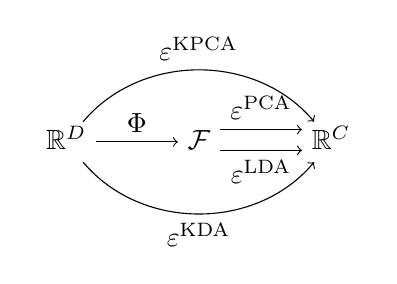
\begin{tikzpicture}
\matrix (m) [matrix of math nodes, row sep=3em,
column sep=3em, text height=1.5ex, text depth=0.25ex]
{ \mathbb{R}^\traceLength & \featureSpace & \mathbb{R}^\newTraceLength \\ };
\path[->]
(m-1-1) edge node[above] {$\Phi$} (m-1-2);
         %edge [bend left=30] (m-2-2)
         %edge [bend right=15] (m-2-2);
\path[->]
($(m-1-2.north east)-(0,0.1)$) edge node[above] {$\extract^{\mathrm{PCA}}$} ($(m-1-3.north west)-(0,0.1)$);
\path[->]
($(m-1-2.south east)+(0,0.15)$) edge node[below] {$\extract^{\mathrm{LDA}}$} ($(m-1-3.south west)+(0,0.15)$);

\path[->]
(m-1-1) edge [bend left=50] node[above] {$\extract^{\mathrm{KPCA}}$} (m-1-3)
(m-1-1) edge [bend right=50] node[below] {$\extract^{\mathrm{KDA}}$} (m-1-3);

\end{tikzpicture} 
}
\end{figure}
\vspace{-10pt}
$\mathcal{F}$ contains all $d$-th degree monomials \small{(dimension increases combinatorially: ${{D}\choose{d}}$)}
\pause

\begin{block}{Kernel function}
 \begin{centering}$K\colon\mathbb{R}^D\times \mathbb{R}^D \rightarrow \mathbb{R} \qquad K(\vLeakVec[]{i},\vLeakVec[]{j}) = \Phi(\vLeakVec[]{i})\cdot \Phi(\vLeakVec[]{j})
$\end{centering}
\end{block}
\pause
\vspace{-5pt}
\begin{block}{Polynomial kernel function}
dth-degree polynomial kernel: $K\colon(\vLeakVec[]{i},\vLeakVec[]{j}) \mapsto ( \vLeakVec[]{i}\cdot \vLeakVec[]{j})^d \leftrightarrow$  all $d$-th degree monomials ($\mathcal{F}$).
\pause

Example: 
$d=2, D=2$; $\vLeakVec[]{i} = [a,b]$ , $\vLeakVec[]{j} = [c,d]$ $\longrightarrow$
\vspace{-10pt}
\begin{equation*}
\textcolor{olive}{K(\vLeakVec[]{i},\vLeakVec[]{j})} = (ac + bd)^2 = a^2c^2 + 2abcd + b^2d^2 \mbox{ ,}
\end{equation*}

%\begin{align}
%&\Phi \colon \mathbb{R}^2 \rightarrow \mathbb{R}^3\\
%&\Phi \colon [a,b]\mapsto [a^2, \sqrt{2}ab, b^2]\\
%&\Phi \colon [c,d]\mapsto [c^2, \sqrt{2}cd, d^2].
%\end{align}
\vspace{-15pt}
\begin{equation*}
K \longleftrightarrow \Phi\colon \Bbb{R}^2\rightarrow\Bbb{R}^3 \qquad \Phi(u,v) =  [u^2, \sqrt{2}uv, v^2]
\end{equation*}
$\textcolor{olive}{\Phi(\vLeakVec[]{i})\cdot \Phi(\vLeakVec[]{j})} = a^2c^2 + 2abcd + b^2d^2 = K(\vLeakVec[]{i},\vLeakVec[]{j})$

\end{block}
\end{frame}

\begin{frame}
[fragile]
\frametitle{LDA to KDA}
\vspace{-30pt}
\begin{figure}
\centering
{
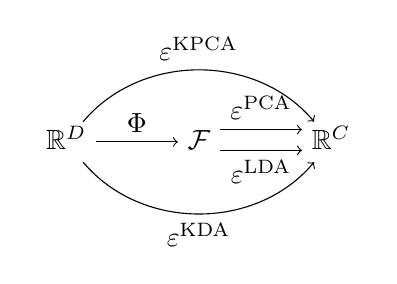
\begin{tikzpicture}
\matrix (m) [matrix of math nodes, row sep=3em,
column sep=3em, text height=1.5ex, text depth=0.25ex]
{ \mathbb{R}^\traceLength & \featureSpace & \mathbb{R}^\newTraceLength \\ };
\path[->]
(m-1-1) edge node[above] {$\Phi$} (m-1-2);
         %edge [bend left=30] (m-2-2)
         %edge [bend right=15] (m-2-2);
\path[->]
($(m-1-2.north east)-(0,0.1)$) edge node[above] {$\extract^{\mathrm{PCA}}$} ($(m-1-3.north west)-(0,0.1)$);
\path[->]
($(m-1-2.south east)+(0,0.15)$) edge node[below] {$\extract^{\mathrm{LDA}}$} ($(m-1-3.south west)+(0,0.15)$);

\path[->]
(m-1-1) edge [bend left=50] node[above] {$\extract^{\mathrm{KPCA}}$} (m-1-3)
(m-1-1) edge [bend right=50] node[below] {$\extract^{\mathrm{KDA}}$} (m-1-3);

\end{tikzpicture} 
}
\end{figure}
\vspace{-15pt}
\begin{columns}
\begin{column}{.5\textwidth}
\begin{block}{LDA}
\begin{itemize}
\item $\AAlpha_i$ eigenvectors of $\SW^{-1}\SB$
\item $\SB$ and $\SW$ depend on data $(\vLeakVec[z_i]{i})$ [$D\times D$]
\item $\extract^{LDA}_{\ell}(\vaLeakVec) = \sum_{i=1}^D \AAlpha_{\ell}[i]\vaLeakVec[i] $
\end{itemize}
\end{block}
\end{column}

\begin{column}{.5\textwidth}
\begin{block}{KDA}
\begin{itemize}
\item $\nununu_i$ eigenvectors of $(\SW^K)^{-1}\SB^K$
\item $\SB^K$ and $\SW^K$ depend on kernel function images $K(\vLeakVec[z_i]{i}, \vLeakVec[z_j]{j})$ [$N\times N$]
\item $\extract^{\mathrm{KDA}}_{\ell}(\vec{x}) = \sum_{i=1}^{\numPoI}\nununu_\ell[i]K(\vLeakVec[z_i]{i}, \vLeakVec[]{}) $
\end{itemize}
\end{block}
\end{column}
\end{columns}
\vspace{-5pt}
\begin{block}{Application Issues}
\begin{itemize}
\item regularization : $\SW^K \leftarrow \SW^K + \mu \III$
\item computational complexity is $O(N^3)$ 
\item non-injective model $\sensVarSet \rightarrow m(\sensVarSet)$ to reduce the number of classes (to improve KDA accuracy in detecting class separating subspaces)
\item asymmetric 'KDA/profiling' approach (to improve profiling accuracy)
\end{itemize}
\end{block}

\end{frame}

\subsection{Experimental Results}


\begin{frame}
\frametitle{Experimental results}
\begin{itemize}
\item $D = 200$: length of rough trace (interesting clock cycles selected)
\item $d=2$, feature extracted from a $200^2 = 40.000$-sized space
\item $d=3 \rightarrow 200^3=6.000.000$ , $d=4 \rightarrow 200^4 = 800.000.000$
\end{itemize}
\begin{figure}[t]

\includegraphics[width=.4\textwidth]{../Figures/CARDIS2016/2order_classes_TA.pdf}
\includegraphics[width=.4\textwidth]{../Figures/CARDIS2016/3order_new.pdf}
\end{figure}
\vspace{-10pt}
\begin{figure}[t]

\includegraphics[width=.4\textwidth]{../Figures/CARDIS2016/3order_2_9.pdf}
\includegraphics[width=.4\textwidth]{../Figures/CARDIS2016/4order_2_9.pdf}
\end{figure}
\end{frame}

\begin{frame}
\frametitle{Limits and Drawbacks}

\end{frame}
%\section{Deep Learning against Misalignment}
\begin{frame}
\frametitle{Contents}
\begin{itemize}
\item \textcolor{grey}{Introduction to LDA: as a classifier, and as a feature extractor
\item Introduction to masking countermeasure and Kernel Discriminant Analysis as a feature extractor}
\item \important{Convolutional Neural Networks and Data Augmentation to attack jitter-based countermeasure}
\end{itemize}
\end{frame}
\begin{frame}
\frametitle{Motivations to apply deep learning techniques}

\end{frame}

\begin{frame}
\frametitle{An integrated approach}
riprendi l'elenco puntato dell'inizio, barra tutto e dici che non si fanno più tanti step ma solo uno\\

più blocco che richiama il teorema di approssimazione universale
\end{frame}

\begin{frame}
\frametitle{Neural Networks}
schema a blocchi con tracce, split in training e validation, passa nel modello, funzione di costo, ottimizzo i pesi, monitoro, re-itero...tante volte..test
\end{frame}

\begin{frame}
\frametitle{Multi-Layer Perceptron}
le couche ...arrivare alla softmax richiamando la spiega sulla LDA

\end{frame}

\begin{frame}

\frametitle{Shift-invariance}
\end{frame}

\begin{frame}
\frametitle{Convolutional Neural Networks}
\end{frame}


\begin{frame}
\frametitle{Our CNN design principle}

\end{frame}


\subsection{Data Augmentation}
\begin{frame}
\frametitle{Data Augmentation}
\vspace{-11pt}
\begin{block}{Data Augmentation}
Artificially generate new training data by deforming those previously acquired,
Applying transformations that preserve the label $\sensRandVar$
\end{block}
\vspace{-5pt}
\begin{block}{Countermeasure Emulation Idea}
Emulate the effects of misaligning countermeasures to generate new traces
\begin{columns}
\begin{column}{0.35\textwidth}
\begin{large}
\textbf{\textcolor{green}{SHIFTING}}
\vspace{-8pt}
\end{large}
\end{column}
\begin{column}{0.35\textwidth}
\begin{large}
\textbf{\textcolor{blue}{ADD-REMOVE}}
\vspace{-8pt}
\end{large}
\end{column}
\end{columns}
\begin{figure}
  \begin{minipage}[b]{0.5\linewidth}
    \centering
    \includegraphics[width=\linewidth]{../Figures/CHES2017/Shifting_window.pdf} 
    \caption{\textcolor{green}{$SH_T$}}
  \end{minipage}%%
  \begin{minipage}[b]{0.5\linewidth}
    \centering
    \includegraphics[width=.7\linewidth]{../Figures/CHES2017/AR_example.pdf} 
    \caption{\textcolor{blue}{$AR_R$}}
  \end{minipage} 
\end{figure}
\vspace{-9pt}
Parameter  \textcolor{green}{$T$}: $\sharp$ of possible positions \hfill \only<2->{\textcolor{red}{\small{$\longrightarrow$ new hyper-parameter}}}\\
Parameter \textcolor{blue}{$R$}: $\sharp$ of added and removed points \hfill \only<2->{\textcolor{red}{\small{$\longrightarrow$ new hyper-parameter}}}\\
Data Augmentation techniques are applied online during training phase.
\end{block}
\end{frame}


\subsection{Experimental Results}
\begin{frame}
\frametitle{Experimental Results}
\begin{itemize}
\item \only<1-2>{Random delays}\only<3>{\textcolor{red}{Random delays}}
\item \only<1-2>{Artificial Jitter}\only<3>{\textcolor{grey}{Artificial Jitter}}
\item \only<1-2>{Real Jitter}\only<3>{\textcolor{red}{Real Jitter}}
\end{itemize}
\uncover<2->{
\begin{block}{}
\begin{itemize}
\item Network architecture: 
$  \softmax \circ [\lambda]^1 \circ[\delta \circ [\sigma \circ \gamma  ]^1 ]^4$

\item Keras library with Tensorflow backend \cite{keras} (open source)
\end{itemize}
\end{block}
}
\end{frame}

\begin{frame}
\vspace*{-5pt}
\frametitle{Random delays}
\vspace{-18pt}
\begin{figure}
\subfloat[One leaking operation]{
\includegraphics[width=.4\textwidth]{../Figures/CHES2017/CW_shift_traces.pdf} }

\end{figure}
\vspace*{-13pt}
\begin{block}{Setup}

\begin{itemize}
\item Target Chip: Atmega328P 
\item Target Variable: $Z = \mathrm{HW}(\mathrm{Sbox}(P\oplus K))$
\item Acquisition: through \emph{ChipWhisperer}\textregistered\ platform, $\approx 4,000$ time samples
\item Countermeasure: Random Delays - insertion of $r$ \emph{nop} operations, $r \in [0,127]$ uniform random
\item $1,000$ training traces

\end{itemize}
\end{block}


\end{frame}

\begin{frame}
\frametitle{Random delays}
\framesubtitle{Data augmentation vs overfitting}
\vspace{-8pt}
\begin{block}{Metrics}
\begin{itemize}
\item Test accuracy: classification accuracy over the attack traces
\item $N^\star$: minimum number of attack traces to make \emph{guessing entropy} of the right key permanently equal to one ($N^\star$ estimated over 10 independent attacks)
\end{itemize}
\end{block}


\begin{figure}
\captionsetup[subfigure]{labelformat=empty}
\subfloat[\textcolor{green}{$SH_0$}]{
\includegraphics[width=.3\textwidth]{../Figures/CHES2017/DAshift0_2000traces_9classes_sgd/acc_DAshift0_2000traces_9classes_sgd.pdf} 
}
\subfloat[\textcolor{green}{$SH_{100}$}]{
\includegraphics[width=.3\textwidth]{../Figures/CHES2017/DAshift100_2000traces_9classes_sgd/acc_DAshift100_2000traces_9classes_sgd.pdf} 
}
\subfloat[\textcolor{green}{$SH_{500}$}]{
\includegraphics[width=.3\textwidth]{../Figures/CHES2017/DAshift500_2000traces_9classes_sgd/acc_DAshift500_2000traces_9classes_sgd.pdf} 
}
\end{figure}

\pause
\vspace*{-15pt}
\begin{table}
\begin{tabular}{|c|c|c|c|c|c|c|c|}
\multicolumn{8}{c}{}\\
\hline
\multicolumn{2}{|c|}{} & \multicolumn{2}{c|}{\textcolor{green}{$\mathrm{SH}_{0}$}} & \multicolumn{2}{c|}{\textcolor{green}{$\mathrm{SH}_{100}$}} & \multicolumn{2}{c|}{\textcolor{green}{$\mathrm{SH}_{500}$}} \\ \hline
Acc        & $N^\star$       & 27.0\%                      & $>1,000$                      & 31.8\%                       & 101                         & \textbf{78\%}              & \textbf{7}                \\ \hline
\end{tabular}
\end{table}
%
\end{frame}
%

\begin{frame}
\frametitle{Random Delays - Two Leaking Operations}

\centering
\includegraphics[width=.5\textwidth]{../Figures/CHES2017/CW_double_shift_traces.pdf}	


\begin{block}{Two leaking operations}
First operation - Test acc: $76.8\%$, $N^\star=7$\\
Second operation - Test acc: $82.5\%$, $N^\star=6$
\end{block}

\end{frame}

\begin{frame}
\frametitle{Artificial Jitter}
\begin{figure}
\subfloat[Low artificial jitter]{\includegraphics[width=.4\textwidth]{../Figures/CHES2017/jitter_2_2_framed.png} }
\subfloat[High artificial jitter]{\includegraphics[width=.4\textwidth]{../Figures/CHES2017/jitter_6_6_framed.png} }
\end{figure}
\begin{block}{Target}

\begin{itemize}
\item Target Variable: $Z = \mathrm{HW}(\mathrm{Sbox}(P\oplus K))$
\item $\approx 2000$ time samples
\item Countermeasure: artificial signal treatment simulating clock jitter
\item 10000 training traces
\end{itemize}
\end{block}


\end{frame}

\begin{frame}
\frametitle{Artificial Jitter (2)}
\vspace*{-10pt}
\begin{scriptsize}
\newcolumntype{C}{>{\centering\arraybackslash}p{3em}}
\begin{table}[t]
\centering

\begin{tabular}{|C|C|CCCCCC|}
\multicolumn{8}{C}{\emph{Low\_jitter}}      \\                                            
\hline
Acc                          & $N^\star$                         & \multicolumn{2}{C|}{$\mathrm{SH}_{0}$}                                                   & \multicolumn{2}{C|}{$\mathrm{SH}_{20}$}                                                & \multicolumn{2}{C|}{$\mathrm{SH}_{40}$}                                           \\ \hline
\multicolumn{2}{|C|}{$\mathrm{AR}_{0}$}   & \multicolumn{1}{C|}{\cellcolor[HTML]{EFEFEF}57.4\%}  & \multicolumn{1}{C|}{\cellcolor[HTML]{EFEFEF}14}     & \multicolumn{1}{C|}{82.5\%}                         & \multicolumn{1}{C|}{6}                              & \multicolumn{1}{C|}{83.6\%}                                  & 6                                                            \\ \cline{1-8}
\multicolumn{2}{|C|}{$\mathrm{AR}_{100}$} & \multicolumn{1}{C|}{86.0\%}                          & \multicolumn{1}{C|}{6}                              & \multicolumn{1}{C|}{87.0\%}                         & \multicolumn{1}{C|}{5}                              & \multicolumn{1}{C|}{87.5\%}                                  & 6                                                             \\ \cline{1-8}
\multicolumn{2}{|C|}{$\mathrm{AR}_{200}$} & \multicolumn{1}{C|}{86.6\%}                          & \multicolumn{1}{C|}{6}                              & \multicolumn{1}{C|}{85.7\%} & \multicolumn{1}{C|}{6}      & \multicolumn{1}{C|}{\textbf{87.7\%}} & \textbf{5}      \\ \hline


\end{tabular}


\end{table}
\begin{table}[t]
\centering


\begin{tabular}{|C|C|CCCCCC|}
\multicolumn{8}{C}{\emph{High\_jitter}}      \\   
\hline
Acc                          & $N^\star$                         & \multicolumn{2}{C|}{$\mathrm{SH}_{0}$}                                                   & \multicolumn{2}{C|}{$\mathrm{SH}_{20}$}                                              & \multicolumn{2}{C|}{$\mathrm{SH}_{40}$}                                             \\ \hline
\multicolumn{2}{|C|}{$\mathrm{AR}_{0}$}   & \multicolumn{1}{C|}{\cellcolor[HTML]{EFEFEF}40.6\%} & \multicolumn{1}{C|}{\cellcolor[HTML]{EFEFEF}35}  & \multicolumn{1}{C|}{51.1\%} & \multicolumn{1}{C|}{9}      & \multicolumn{1}{C|}{62.4\%}           & 11                                 \\ \cline{1-8}
\multicolumn{2}{|C|}{$\mathrm{AR}_{100}$} & \multicolumn{1}{C|}{50.2\%} & \multicolumn{1}{C|}{15}     & \multicolumn{1}{C|}{72.4\%} & \multicolumn{1}{C|}{11}     & \multicolumn{1}{C|}{73.5\%}           & 9                       \\ \cline{1-8}
\multicolumn{2}{|C|}{$\mathrm{AR}_{200}$} & \multicolumn{1}{C|}{64.0\%} & \multicolumn{1}{C|}{11}     & \multicolumn{1}{C|}{\textbf{75.5\%}} & \multicolumn{1}{C|}{\textbf{8}}   & \multicolumn{1}{C|}{74.4\%}           & 8           \\ \hline


\end{tabular}


\end{table}
\end{scriptsize}


\begin{figure}
\subfloat[Low Jitter]{\includegraphics[width=.45\textwidth]{../Figures/CHES2017/results_low_jitter_new.pdf} }
\subfloat[High Jitter]{\includegraphics[width=.45\textwidth]{../Figures/CHES2017/results_high_jitter_new.pdf} }

\end{figure}
\end{frame}



\begin{frame}
\frametitle{Artificial Jitter}
\begin{tiny}

\newcolumntype{C}{>{\centering\arraybackslash}p{3em}}
\begin{table}[t]
\centering
\label{table:results_all}



\begin{tabular}{|C|C|CCCCCC|CC}
\hline
\multicolumn{10}{|C|}{\textbf{\emph{DS\_low\_jitter}}}\\
\hline
$a$                           & $b$                         & \multicolumn{2}{C|}{}                                                                                      & \multicolumn{2}{C|}{}                                                                                     & \multicolumn{2}{C|}{}                                                                                  & \multicolumn{2}{C|}{}                                      \\ \cline{1-2}
$c$                           & $d$                         & \multicolumn{2}{C|}{\multirow{-2}{*}{$\mathrm{SH}_{0}$}}                                                   & \multicolumn{2}{c|}{\multirow{-2}{*}{$\mathrm{SH}_{20}$}}                                                 & \multicolumn{2}{c|}{\multirow{-2}{*}{$\mathrm{SH}_{40}$}}                                              & \multicolumn{2}{c|}{\multirow{-2}{*}{$\mathrm{SH}_{200}$}} \\ \hline
\multicolumn{2}{|c|}{}                                      & \multicolumn{1}{c|}{\cellcolor[HTML]{EFEFEF}100.0\%} & \multicolumn{1}{c|}{\cellcolor[HTML]{EFEFEF}68.7\%} & \multicolumn{1}{c|}{99.8\%}                         & \multicolumn{1}{c|}{86.1\%}                         & \multicolumn{1}{c|}{98.9\%}                                  & 84.1\%                                  &                              &                             \\ \cline{3-8}
\multicolumn{2}{|c|}{\multirow{-2}{*}{$\mathrm{AR}_{0}$}}   & \multicolumn{1}{c|}{\cellcolor[HTML]{EFEFEF}57.4\%}  & \multicolumn{1}{c|}{\cellcolor[HTML]{EFEFEF}14}     & \multicolumn{1}{c|}{82.5\%}                         & \multicolumn{1}{c|}{6}                              & \multicolumn{1}{c|}{83.6\%}                                  & 6                                       &                              &                             \\ \cline{1-8}
\multicolumn{2}{|c|}{}                                      & \multicolumn{1}{c|}{87.7\%}                          & \multicolumn{1}{c|}{88.2\%}                         & \multicolumn{1}{c|}{82.4\%}                         & \multicolumn{1}{c|}{88.4\%}                         & \multicolumn{1}{c|}{81.9\%}                                  & 89.6\%                                  &                              &                             \\ \cline{3-8}
\multicolumn{2}{|c|}{\multirow{-2}{*}{$\mathrm{AR}_{100}$}} & \multicolumn{1}{c|}{86.0\%}                          & \multicolumn{1}{c|}{6}                              & \multicolumn{1}{c|}{87.0\%}                         & \multicolumn{1}{c|}{5}                              & \multicolumn{1}{c|}{87.5\%}                                  & 6                                       &                              &                             \\ \cline{1-8}
\multicolumn{2}{|c|}{}                                      & \multicolumn{1}{c|}{83.2\%}                          & \multicolumn{1}{c|}{88.6\%}                         & \multicolumn{1}{c|}{81.4\%} & \multicolumn{1}{c|}{86.9\%} & \multicolumn{1}{c|}{\textbf{80.6\%}} &\textbf{88.9\%} &                              &                             \\ \cline{3-8}
\multicolumn{2}{|c|}{\multirow{-2}{*}{$\mathrm{AR}_{200}$}} & \multicolumn{1}{c|}{86.6\%}                          & \multicolumn{1}{c|}{6}                              & \multicolumn{1}{c|}{85.7\%} & \multicolumn{1}{c|}{6}      & \multicolumn{1}{c|}{\textbf{87.7\%}} & \textbf{5}      &                              &                             \\ \hline
\multicolumn{2}{|c|}{}                                      &                                                      &                                                     &                                                     &                                                     &                                                              &                                         & \multicolumn{1}{c|}{85.0\%}  & \multicolumn{1}{c|}{88.6\%} \\ \cline{9-10} 
\multicolumn{2}{|c|}{\multirow{-2}{*}{$\mathrm{AR}_{500}$}} &                                                      &                                                     &                                                     &                                                     &                                                              &                                         & \multicolumn{1}{c|}{86.2\%}  & \multicolumn{1}{c|}{5}      \\ \cline{1-2} \cline{9-10}
\multicolumn{10}{|C|}{}\\
\hline
\multicolumn{10}{|C|}{\textbf{\emph{DS\_high\_jitter}}}\\
\hline
$a$                          & $b$                         & \multicolumn{2}{C|}{\multirow{2}{*}{$\mathrm{SH}_{0}$}}   & \multicolumn{2}{C|}{\multirow{2}{*}{$\mathrm{SH}_{20}$}}  & \multicolumn{2}{C|}{\multirow{2}{*}{$\mathrm{SH}_{40}$}} & \multicolumn{2}{C|}{\multirow{2}{*}{$\mathrm{SH}_{200}$}} \\ \cline{1-2}
$c$                          & $d$                         & \multicolumn{2}{C|}{}                                     & \multicolumn{2}{C|}{}                                     & \multicolumn{2}{C|}{}                                    & \multicolumn{2}{C|}{}                                     \\ \hline
\multicolumn{2}{|C|}{\multirow{2}{*}{$\mathrm{AR}_{0}$}}   & \multicolumn{1}{C|}{\cellcolor[HTML]{EFEFEF}100\%}  & \multicolumn{1}{l|}{\cellcolor[HTML]{EFEFEF}45.0\%} & \multicolumn{1}{C|}{100\%}  & \multicolumn{1}{C|}{60.0\%} & \multicolumn{1}{l|}{98.5\%}           & 67.6\%           &                             &                             \\ \cline{3-8}
\multicolumn{2}{|C|}{}                                     &  \multicolumn{1}{C|}{\cellcolor[HTML]{EFEFEF}40.6\%} & \multicolumn{1}{C|}{\cellcolor[HTML]{EFEFEF}35}  & \multicolumn{1}{C|}{51.1\%} & \multicolumn{1}{C|}{9}      & \multicolumn{1}{C|}{62.4\%}           & 11               &                             &                             \\ \cline{1-8}
\multicolumn{2}{|C|}{\multirow{2}{*}{$\mathrm{AR}_{100}$}} & \multicolumn{1}{C|}{90.4\%} & \multicolumn{1}{l|}{57.3\%} & \multicolumn{1}{C|}{76.6\%} & \multicolumn{1}{C|}{73.6\%} & \multicolumn{1}{C|}{78.5\%}           & 76.4\%           &                             &                             \\ \cline{3-8}
\multicolumn{2}{|C|}{}                                     & \multicolumn{1}{C|}{50.2\%} & \multicolumn{1}{C|}{15}     & \multicolumn{1}{C|}{72.4\%} & \multicolumn{1}{C|}{11}     & \multicolumn{1}{C|}{73.5\%}           & 9                &                             &                             \\ \cline{1-8}
\multicolumn{2}{|C|}{\multirow{2}{*}{$\mathrm{AR}_{200}$}} & \multicolumn{1}{C|}{83.1\%} & \multicolumn{1}{C|}{67.7\%} &\multicolumn{1}{C|}{\textbf{82.0\%}} & \multicolumn{1}{C|}{\textbf{77.1\%}} & \multicolumn{1}{l|}{82.6\%}           & 77.0\%           &                             &                             \\ \cline{3-8}
\multicolumn{2}{|C|}{}                                     & \multicolumn{1}{C|}{64.0\%} & \multicolumn{1}{C|}{11}     & \multicolumn{1}{C|}{\textbf{75.5\%}} & \multicolumn{1}{C|}{\textbf{8}}   & \multicolumn{1}{C|}{74.4\%}           & 8                &                             &                             \\ \hline
\multicolumn{2}{|C|}{\multirow{2}{*}{$\mathrm{AR}_{500}$}} &                             &                             &                             &                             &                                       &                  & \multicolumn{1}{C|}{83.6\%} & \multicolumn{1}{C|}{73.4\%} \\ \cline{9-10} 
\multicolumn{2}{|C|}{}                                     &                             &                             &                             &                             &                                       &                  & \multicolumn{1}{C|}{68.2\%} & \multicolumn{1}{C|}{11}     \\ \cline{1-2} \cline{9-10}  
\end{tabular}


\end{table}

\end{tiny}
\end{frame}

\begin{frame}
\frametitle{Real Jitter (1)}
\vspace{-10pt}
\begin{block}{Target}
\begin{itemize}
\item AES hardware implementation
\item strong jitter effect
\item Target Variable: $Z = \mathrm{Sbox}(P\oplus K)$
\item $2,500$ selected time samples
\item $99,000$ training traces
\end{itemize}
\end{block}

\only<1>{
\includegraphics[width=\textwidth]{../Figures/CHES2017/SNR_firstSbox.pdf}
}
\only<2>{
\includegraphics[width=\textwidth]{../Figures/CHES2017/SNR_desynchro.pdf}
}



\end{frame}

\begin{frame}
\frametitle{Real Jitter (2)}
\centering
\begin{scriptsize}
\begin{table}
\begin{tabular}{|c|c|c|c|c|c|c|c|}
\multicolumn{8}{c}{}\\
\hline
\multicolumn{2}{|c|}{} & \multicolumn{2}{c|}{\textcolor{green}{$\mathrm{SH}_{0}$}\textcolor{blue}{$\mathrm{AR}_{0}$}} & \multicolumn{2}{c|}{\textcolor{green}{$\mathrm{SH}_{10}$}\textcolor{blue}{$\mathrm{AR}_{100}$}} & \multicolumn{2}{c|}{\textcolor{green}{$\mathrm{SH}_{20}$}\textcolor{blue}{$\mathrm{AR}_{200}$}} \\ \hline
Acc        & $N^\star$       & 1.2\%                      & 137                      & 1.3\%                       & 89                         & \textbf{1.8\%}              & \textbf{54}                \\ \hline
\end{tabular}
\end{table}
\end{scriptsize}
\uncover<2>{
\includegraphics[width=0.75\textwidth]{../Figures/CHES2017/SNR_resynchro.pdf} 
}
\vspace*{-18pt}

\centering
\uncover<2>{
\includegraphics[width=0.5\textwidth]{../Figures/CHES2017/TA_CNN_smartcard.pdf} 
}


\end{frame}


\section*{Conclusions}

\begin{frame}
\begin{block}{\textit{Today}}
\begin{itemize}
\item suites de la KDA
\item ASCAD plus toutes les contributions CNN sorties dernieremets
\end{itemize}
\end{block}
\end{frame}
%\begin{frame}
%\frametitle{Conclusions}
%\begin{block}{Conclusions}
%\begin{itemize}
%\item Projecting extractors for dimensionality reduction of side-channel traces
%\item Contribution to the components selection problem (ELV) 
%\item[][Paper accepted at \emph{CARDIS 2015} international conference]
%\item Proposal and validation of KDA technique with $d$th-degree polynomial kernel to extract information in presence of $(d-1)$th sharing countermeasure 
%\item[][Paper accepted at \emph{CARDIS 2016} international conference]
%\end{itemize}
%\end{block}
%
%\hfill
%\begin{huge}
%Thank You!
%\end{huge}
%%\begin{block}{Future Works}
%%\begin{itemize}
%%\item Gaussian Template Attacks: exploit linear regression model to raise the accuracy of the template estimations
%%\item Convolutional Neural Networks: construct networks adapted to SCAs 
%%\end{itemize}
%%\end{block}
%
%\end{frame}





\backupbegin

\begin{frame}[allowframebreaks]
\frametitle{References}
\printbibliography
\end{frame}


%\begin{frame}\frametitle{Setup and Implementation}
%Target device and acquisitions: 
%
%\begin{itemize}
%\item 8-bit AVR microprocessor Atmega328P
%\item power-consumption acquired via the ChipWhisperer \cite{o2014chipwhisperer} platform
%\end{itemize}
%
%
%
%Implementation: 
%
%\begin{itemize}
%\item Begin of an AES-128
%\end{itemize}
%
%
%
%Attack: 
%
%
%\begin{itemize}
%\item Target sensitive variable: $Z = \mathrm{Sbox}(P_0 \oplus K_0)$
%\item Acquisition of $N_p\times 256$ profiling traces, under key knowledge
%\item Estimation of $C$-dimensional Gaussian templates via the projection of the profiling traces over the $C$ projecting components
%\item Template attack with $N$ attack traces
%\end{itemize}
%
%\end{frame}
%
%
%\begin{frame} \frametitle{The Problem of Selecting PCA Components - EGV}
%
%% state of the art
%% first and sixth PC DPA contest
%\begin{columns}
%\begin{column}{0.1\textwidth}
%\includegraphics[width = \textwidth]{figures/questionmark.jpg} 
%\end{column}
%\begin{column}{0.7\textwidth}
%\begin{block}{}
%{\em How many} PCs and {\em which ones} are sufficient/necessary to reduce the traces size without losing important discriminant information?
%\end{block}
%\end{column}
%\end{columns}
%\pause
%\begin{block}{Explained Global Variance (EGV)}
%$\EGV{\AAlpha_i} = \frac{\lambda_i}{\sum_{k=1}^r \lambda_k}$\\
%\cite{choudaryefficient} : 
%\begin{itemize}
%\item fix a threshold $\beta$
%\item choose the first $C$ components, where $C$ is the minimum integer such that
%\begin{equation*}
%\EGV{\AAlpha_1}+ \EGV{\AAlpha_2}+\dots + \EGV{\AAlpha_C} \geq \beta
%\end{equation*}
%\end{itemize}
%\end{block}
%
%
%
%\end{frame}
%
%
%\begin{frame} \frametitle{The Problem of Selecting PCA Components - Experimental Observation}
%\begin{block}{Experimental Observation}
%\cite{Batina2012,specht}: the first components sometimes contain more noise than information; it is worth discarding them.
%\end{block}
%\begin{figure}
%\includegraphics[width=.45\textwidth]{figures/DPAcontestPC1_new.pdf} 
%\includegraphics[width=.45\textwidth]{figures/DPAcontestPC6_new.pdf} 
%\caption{First and sixth PCs in DPA contest v4  \cite{DPAcontest} trace set}\label{fig:DPAcontest}
%\end{figure}
%\end{frame}
%
%\begin{frame} \frametitle{The Problem of Selecting PCA Components - IPR}
%\begin{block}{Assumption}
%Dealing with secured devices, the leaking side-channel information is localised in few points of the acquired trace.
%\end{block}
%\pause
%\begin{block}{Inverse Participation Ratio (IPR)}
%\cite{SCAclassProbl}: under the same assumption, use the IPR to choose informative components
%\begin{equation*}
%\mathrm{IPR}(\AAlpha_i) = \sum_{j=1}^\traceLength \AAlpha_i[j]^4 \mbox{ \em (localization score)}
%\end{equation*}
%\end{block}
%\end{frame}
%
%\begin{frame} \frametitle{The Explained Local Variance (ELV) Selection (1)}
%
%What minds to perform the choice of the PCs to keep:
%\begin{table}
%\begin{tabular}{|c|c|c|c|}
%\hline
%& EGV & IPR & \uncover<2->{\textbf{ELV}} \\
%\hline
%associated eigenvalue ($\lambda_i$) &\includegraphics[scale=0.01]{figures/yes.png}  & \includegraphics[scale=0.01]{figures/no.png} &\uncover<2->{\includegraphics[scale=0.015]{figures/yes.png}}\\
%\hline
%component form (localization of $\AAlpha_i$) &\includegraphics[scale=0.01]{figures/no.png}  & \includegraphics[scale=0.01]{figures/yes.png}&\uncover<2->{\includegraphics[scale=0.015]{figures/yes.png}} \\
%\hline
%\end{tabular}
%\end{table}
%
%\uncover<3->{
%\begin{block}{Inspection of $\lambda_i$}
%\begin{scriptsize}
%
%\begin{align*}
%\lambda_i =& \textcolor{gray}{\hat{\mathrm{var}}(\sum_{j=1}^D \XXX^\intercal[j]\AAlpha_i[j]) = \sum_{j=1}^D\sum_{k=1}^D \hat{\mathrm{cov}}(\XXX^\intercal[j]\AAlpha_i[j], \XXX^\intercal[k]\AAlpha_i[k])=}\\
%\textcolor{gray}{=}& \textcolor{gray}{\sum_{j=1}^D \AAlpha_i[j]\sum_{k=1}^D\AAlpha_i[k]\hat{\mathrm{cov}}(\XXX^\intercal[j], \XXX^\intercal[k])= \sum_{j=1}^D \AAlpha_i[j] (\covmat_{j}^\intercal \cdot \AAlpha_i)= } \\
%\textcolor{gray}{=}& \textcolor{gray}{\sum_{j=1}^D \AAlpha_i[j] \lambda_i\AAlpha_i[j] }= \sum_{j=1}^D  \lambda_i \AAlpha_i[j]^2 
%\end{align*}
%\end{scriptsize}
%
%The $j$-th time sample contribution to $\lambda_i$ is given by $\lambda_i \AAlpha_i[j]^2$
%\end{block}
%}
%
%
%\end{frame}
%
%\begin{frame} \frametitle{The ELV Selection (2)}
%\vspace*{-0.5cm}
%\uncover<1->{
%\begin{block}{Definition}
%$\mathrm{ELV}(\AAlpha_i,j) = \frac{\lambda_i \AAlpha_i[j]^2}{\sum_{k=1}^r\lambda_k} = \mathrm{EGV}(\AAlpha_i) \AAlpha_i[j]^2$  \\
%\uncover<2->{Observe that $\sum_{j=1}^D \mathrm{ELV}(\AAlpha_i,j) = \EGV{\AAlpha_i}$}
%\end{block}
%}
%\uncover<3->{
%Perform this sum in a cumulative way, sorting the ELV contributions of the time samples in decreasing order, {\em i. e.} $\mathrm{ELV}(\AAlpha_i,j^i_1)\geq \mathrm{ELV}(\AAlpha_i,j^i_2)\geq \dots \geq \mathrm{ELV}(\AAlpha_i,j^i_\traceLength)$
%
%
%\vspace*{-0.4cm}
%\begin{columns}
%\begin{column}{.5\textwidth}
%\vspace*{10pt}
%\begin{figure}
%\includegraphics[width=\textwidth]{figures/PC1_points.pdf} 
%\end{figure}
%\end{column}
%\begin{column}{.5\textwidth}
%\begin{figure}
%
%\begin{tikzpicture}[remember picture,
%    scale=1,
%    % Define styles here
%    every node/.style={transform shape}
%    block/.style={
%        rectangle,
%        draw,
%        text centered,
%        rounded corners
%        },
%    data/.style={
%        trapezium,
%        trapezium left angle=60,
%        trapezium right angle=120,
%        draw
%        },
%    component/.style={
%        circle,
%        draw
%        },
%    output/.style={
%        tape,
%        tape bend top=none,
%        draw
%        },
%    edge/.style={
%        ->,
%        >=stealth,
%        thick
%        }
%    ]
%
%    \node (only1elv) at (0,0)
%    {\includegraphics[width=\textwidth]{figures/cumulativeELV_only1.pdf} };
%    \node [component, thick, xshift=2.1cm, yshift=0.8cm] (cerchio) {};
%    \node[below left=1cm of cerchio](caption){$\mathrm{EGV}(\AAlpha_1)$};
%    \draw[->] (caption) to (cerchio.south west);
%\end{tikzpicture}
%\end{figure}
%\end{column}
%\end{columns}
%
%
%}
%
%\end{frame}
%
%
%
%\begin{frame}
%\frametitle{The ELV Selection (3)}
%\begin{columns}
%\begin{column}{0.5\textwidth}
%\uncover<1->{
%\only<1>{
%\vspace*{-0.4cm}
%\begin{center}
%\includegraphics[width = \textwidth]{figures/cumulativeELV.pdf}
%\end{center}
%}
%\only<2>{
%\vspace*{-0.4cm}
%\begin{center}
%\includegraphics[width = \textwidth]{figures/cumulativeELVallRectangle.pdf} 
%\end{center}
%}
%
%\only<3->{
%\vspace*{-0.4cm}
%\begin{center}
%\includegraphics[width = \textwidth]{figures/cumulativeELVzoomed.pdf}
%\end{center}
%}
%}
%\uncover<4->{
%\only<1-4>{
%
%\begin{block}{To select $C$ components\hspace{\textwidth}\textcolor{white}{ }}
%Sort in decreasing order the maximal ELV provided by each component $\{\max_{j=1,\dots,D}\ELV(\AAlpha_i,j)\}_{i}$ and select the $C$ first components.
%\end{block}
%}
%\only<5>{
%
%\begin{block}{Fixing a cumulative explained variance threshold $\beta$}
%Select \textbf{couples} $(\AAlpha_i, j)$ in decreasing order wrt to $\ELV(\AAlpha_i, j)$ until $\ELV(\AAlpha_{i_1}, j_1)+ \ELV(\AAlpha_{i_2}, j_2)+\dots +\ELV(\AAlpha_{i_M}, j_M)\geq \beta$.\\
%%\uncover<5>{{\em Components denoising}}
%\end{block}
%}
%}
%
%\end{column}
%
%\begin{column}{0.5\textwidth}
%\only<1-3>{
%\begin{figure}
%\includegraphics[width=0.5\textwidth]{figures/PC1.pdf} 
%\includegraphics[width=0.5\textwidth]{figures/PC4.pdf} \\
%\includegraphics[width=0.5\textwidth]{figures/PC2.pdf} 
%\includegraphics[width=0.5\textwidth]{figures/PC5.pdf} \\
%\includegraphics[width=0.5\textwidth]{figures/PC3.pdf} 
%\includegraphics[width=0.5\textwidth]{figures/PC6.pdf} 
%\caption{\begin{footnotesize}
%The first 6 PCs: 
%$\lambda_1 \approx 3.8 ,\lambda_2 \approx 3.1 , \lambda_3 \approx2.6 ,\lambda_4 \approx 1.0 ,\lambda_5 \approx 0.8 ,\lambda_6 \approx 0.6 $
%\end{footnotesize}}
%
%\end{figure}
%}
%
%
%\only<4-5>{
%\begin{figure}
%\onslide<5->{\includegraphics[width=0.5\textwidth]{figures/PC5_denoised.pdf}}\only<4>{\includegraphics[width=0.5\textwidth]{figures/PC5_cerchio.pdf}}\only<5>{\includegraphics[width=0.5\textwidth]{figures/PC5_cerchio_transp.pdf}} \\
%\onslide<5->{\includegraphics[width=0.5\textwidth]{figures/PC4_denoised.pdf}}\only<4>{\includegraphics[width=0.5\textwidth]{figures/PC4_cerchio.pdf}}\only<5>{\includegraphics[width=0.5\textwidth]{figures/PC4_cerchio_transp.pdf}} \\
%\onslide<5->{\includegraphics[width=0.5\textwidth]{figures/PC6_denoised.pdf}}\only<4>{\includegraphics[width=0.5\textwidth]{figures/PC6_cerchio.pdf}}\only<5>{\includegraphics[width=0.5\textwidth]{figures/PC6_cerchio_transp.pdf}} 
%\only<4>{\caption{The 3 components chosen by ELV selection method - $C$ fixed}}
%\only<5>{\caption{Components and time samples chosen by ELV selection method - $\beta$ fixed}}
%\end{figure}
%}
%
%
%%\only<5>{
%%\includegraphics[width=0.31\textwidth]{ figures/PC5_cerchio_transp.pdf} 
%%\includegraphics[width=0.31\textwidth]{ figures/PC4_cerchio_transp.pdf} 
%%\includegraphics[width=0.31\textwidth]{ figures/PC6_cerchio_transp.pdf} \\
%%}
%%\uncover<5>{
%%
%%
%%
%%\only<3-4>{\caption{Selected components for $C = 3$; \hspace{\textwidth} $\ELV(\AAlpha_5, 2362)\approx 0.41$, $\ELV(\AAlpha_4, 1110)\approx 0.38$, $\ELV(\AAlpha_6, 1118)\approx 0.24$}}
%%\only<5>{\caption{Selected and denoised components for $\beta = 0.08$\hspace{\textwidth}\textcolor{white}{$\ELV(\AAlpha_5, 2362)\approx 0.41$, $\ELV(\AAlpha_4, 1110)\approx 0.38$, $\ELV(\AAlpha_6, 1118)\approx 0.24$}}}
%
%\end{column}
%
%\end{columns}
%
%
%\end{frame}
%
%%\begin{frame} \frametitle{The Component Selection Issue}
%%
%%\begin{columns}
%%\begin{column}{0.1\textwidth}
%%\includegraphics[width = \textwidth]{figures/questionmark.jpg} 
%%\end{column}
%%\begin{column}{0.7\textwidth}
%%\begin{block}{}
%%{\em How many} PCs and {\em which ones} are sufficient/necessary to reduce the traces size without losing important discriminant information? 
%%\end{block}
%%\end{column}
%%\end{columns}
%% \only<1>{
%% \begin{block}{Theoretically}
%%Higher eigenvalues $\longrightarrow$ higher information.
%%\end{block}
%%\begin{block}{Experimental Observation}
%%\cite{Batina2012,specht}: the first components sometimes contain no sensitive information; it is worth discarding them.
%%\end{block}
%%
%%\begin{figure}
%%\includegraphics[width=.25\textwidth]{figures/DPAcontestPC1_new.pdf} 
%%\includegraphics[width=.25\textwidth]{figures/DPAcontestPC6_new.pdf} 
%%\vspace{-10pt}
%%\caption{First and sixth PCs in DPA contest v4  \cite{DPAcontest} trace set}\label{fig:DPAcontest}
%%\end{figure}
%%}
%%\only<2>{
%%\vspace{40pt}
%%\begin{small}
%%\begin{table}
%%\begin{tabular}{|c|c|c|c|}
%%\hline
%%& EGV \cite{choudaryefficient} & IPR \cite{SCAclassProbl}& \uncover<2->{\textbf{ELV} \cite{Cagli2016}} \\
%%\hline
%%eigenvalue $\lambda_i$ &\includegraphics[scale=0.01]{figures/yes.png}  & \includegraphics[scale=0.01]{figures/no.png} &\uncover<2->{\includegraphics[scale=0.015]{figures/yes.png}}\\
%%\hline
%%form of $\AAlpha_i$ &\includegraphics[scale=0.01]{figures/no.png}  & \includegraphics[scale=0.01]{figures/yes.png}&\uncover<2->{\includegraphics[scale=0.015]{figures/yes.png}} \\
%%\hline
%%\end{tabular}
%%\end{table}
%%\end{small}
%%
%%\includegraphics[scale=0.3]{figures/citazione1.jpg} 
%%}
%%\uncover<2->{
%%\begin{block}{Explained Local Variance}
%%$\mathrm{ELV}(\AAlpha_i,j) = \frac{\lambda_i \AAlpha_i[j]^2}{\sum_{k=1}^r\lambda_k} = \mathrm{EGV}(\AAlpha_i) \AAlpha_i[j]^2$  \\
%%%($\sum_{j=1}^D \mathrm{ELV}(\AAlpha_i,j) = \EGV{\AAlpha_i}$)
%%\end{block}
%%}
%%\uncover<3->{\begin{block}{Use of the ELV}
%%\begin{itemize}
%%\item Sort in decreasing order the maximal ELV provided by each component $\{\max_{j=1,\dots,D}\ELV(\AAlpha_i,j)\}_{i}$ and select the $C$ first components.
%%\item Select \textbf{couples} $(\AAlpha_i, j)$ in decreasing order wrt to $\ELV(\AAlpha_i, j)$ until $\ELV(\AAlpha_{i_1}, j_1)+ \ELV(\AAlpha_{i_2}, j_2)+\dots +\ELV(\AAlpha_{i_M}, j_M)\geq \beta$
%%\end{itemize}
%%\end{block}}
%%\end{frame}
%%
%%\begin{frame} \frametitle{The ELV Selection (2)}
%%\vspace*{-0.5cm}
%%\uncover<1->{
%%\begin{block}{Definition}
%%$\mathrm{ELV}(\AAlpha_i,j) = \frac{\lambda_i \AAlpha_i[j]^2}{\sum_{k=1}^r\lambda_k} = \mathrm{EGV}(\AAlpha_i) \AAlpha_i[j]^2$  \\
%%\uncover<2->{Observe that $\sum_{j=1}^D \mathrm{ELV}(\AAlpha_i,j) = \EGV{\AAlpha_i}$}
%%\end{block}
%%}
%%\uncover<3->{
%%Perform this sum in a cumulative way, sorting the ELV contributions of the time samples in decreasing order, {\em i. e.} $\mathrm{ELV}(\AAlpha_i,j^i_1)\geq \mathrm{ELV}(\AAlpha_i,j^i_2)\geq \dots \geq \mathrm{ELV}(\AAlpha_i,j^i_\traceLength)$
%%
%%
%%\vspace*{-0.4cm}
%%\begin{columns}
%%\begin{column}{.5\textwidth}
%%\vspace*{10pt}
%%\begin{figure}
%%\includegraphics[width=\textwidth]{figures/PC1_points.pdf} 
%%\end{figure}
%%\end{column}
%%\begin{column}{.5\textwidth}
%%\begin{figure}
%%
%%\begin{tikzpicture}[remember picture,
%%    scale=1,
%%    % Define styles here
%%    every node/.style={transform shape}
%%    block/.style={
%%        rectangle,
%%        draw,
%%        text centered,
%%        rounded corners
%%        },
%%    data/.style={
%%        trapezium,
%%        trapezium left angle=60,
%%        trapezium right angle=120,
%%        draw
%%        },
%%    component/.style={
%%        circle,
%%        draw
%%        },
%%    output/.style={
%%        tape,
%%        tape bend top=none,
%%        draw
%%        },
%%    edge/.style={
%%        ->,
%%        >=stealth,
%%        thick
%%        }
%%    ]
%%
%%    \node (only1elv) at (0,0)
%%    {\includegraphics[width=\textwidth]{figures/cumulativeELV_only1.pdf} };
%%    \node [component, thick, xshift=2.1cm, yshift=0.8cm] (cerchio) {};
%%    \node[below left=1cm of cerchio](caption){$\mathrm{EGV}(\AAlpha_1)$};
%%    \draw[->] (caption) to (cerchio.south west);
%%\end{tikzpicture}
%%\end{figure}
%%\end{column}
%%\end{columns}
%%
%%
%%}
%%
%%\end{frame}
%%
%%
%%
%%%\begin{frame}
%%\frametitle{The ELV Selection (2)}
%%\begin{columns}
%%\begin{column}{0.5\textwidth}
%%\uncover<1->{
%%\only<1>{
%%\vspace*{-0.4cm}
%%\begin{center}
%%\includegraphics[width = \textwidth]{figures/cumulativeELV.pdf}
%%\end{center}
%%}
%%\only<2>{
%%\vspace*{-0.4cm}
%%\begin{center}
%%\includegraphics[width = \textwidth]{figures/cumulativeELVallRectangle.pdf} 
%%\end{center}
%%}
%%
%%\only<3->{
%%\vspace*{-0.4cm}
%%\begin{center}
%%\includegraphics[width = \textwidth]{figures/cumulativeELVzoomed.pdf}
%%\end{center}
%%}
%%}
%%\uncover<4->{
%%\only<1-4>{
%%
%%\begin{block}{To select $C$ components\hspace{\textwidth}\textcolor{white}{ }}
%%Sort in decreasing order the maximal ELV provided by each component $\{\max_{j=1,\dots,D}\ELV(\AAlpha_i,j)\}_{i}$ and select the $C$ first components.
%%\end{block}
%%}
%%\only<5>{
%%
%%\begin{block}{Fixing a cumulative explained variance threshold $\beta$}
%%Select \textbf{couples} $(\AAlpha_i, j)$ in decreasing order wrt to $\ELV(\AAlpha_i, j)$ until $\ELV(\AAlpha_{i_1}, j_1)+ \ELV(\AAlpha_{i_2}, j_2)+\dots +\ELV(\AAlpha_{i_M}, j_M)\geq \beta$.\\
%%%\uncover<5>{{\em Components denoising}}
%%\end{block}
%%}
%%}
%%
%%\end{column}
%%
%%\begin{column}{0.5\textwidth}
%%\only<1-3>{
%%\begin{figure}
%%\includegraphics[width=0.5\textwidth]{figures/PC1.pdf} 
%%\includegraphics[width=0.5\textwidth]{figures/PC4.pdf} \\
%%\includegraphics[width=0.5\textwidth]{figures/PC2.pdf} 
%%\includegraphics[width=0.5\textwidth]{figures/PC5.pdf} \\
%%\includegraphics[width=0.5\textwidth]{figures/PC3.pdf} 
%%\includegraphics[width=0.5\textwidth]{figures/PC6.pdf} 
%%\caption{\begin{footnotesize}
%%The first 6 PCs: 
%%$\lambda_1 \approx 3.8 ,\lambda_2 \approx 3.1 , \lambda_3 \approx2.6 ,\lambda_4 \approx 1.0 ,\lambda_5 \approx 0.8 ,\lambda_6 \approx 0.6 $
%%\end{footnotesize}}
%%
%%\end{figure}
%%}
%%
%%
%%\only<4-5>{
%%\begin{figure}
%%\onslide<5->{\includegraphics[width=0.5\textwidth]{figures/PC5_denoised.pdf}}\only<4>{\includegraphics[width=0.5\textwidth]{figures/PC5_cerchio.pdf}}\only<5>{\includegraphics[width=0.5\textwidth]{figures/PC5_cerchio_transp.pdf}} \\
%%\onslide<5->{\includegraphics[width=0.5\textwidth]{figures/PC4_denoised.pdf}}\only<4>{\includegraphics[width=0.5\textwidth]{figures/PC4_cerchio.pdf}}\only<5>{\includegraphics[width=0.5\textwidth]{figures/PC4_cerchio_transp.pdf}} \\
%%\onslide<5->{\includegraphics[width=0.5\textwidth]{figures/PC6_denoised.pdf}}\only<4>{\includegraphics[width=0.5\textwidth]{figures/PC6_cerchio.pdf}}\only<5>{\includegraphics[width=0.5\textwidth]{figures/PC6_cerchio_transp.pdf}} 
%%\only<4>{\caption{The 3 components chosen by ELV selection method - $C$ fixed}}
%%\only<5>{\caption{Components and time samples chosen by ELV selection method - $\beta$ fixed}}
%%\end{figure}
%%}
%%
%%
%%\only<5>{
%%\includegraphics[width=0.31\textwidth]{figures/PC5_cerchio_transp.pdf} 
%%\includegraphics[width=0.31\textwidth]{figures/PC4_cerchio_transp.pdf} 
%%\includegraphics[width=0.31\textwidth]{figures/PC6_cerchio_transp.pdf} \\
%%}
%%\uncover<5>{
%%
%%
%%
%%\only<3-4>{\caption{Selected components for $C = 3$; \hspace{\textwidth} $\ELV(\AAlpha_5, 2362)\approx 0.41$, $\ELV(\AAlpha_4, 1110)\approx 0.38$, $\ELV(\AAlpha_6, 1118)\approx 0.24$}}
%%\only<5>{\caption{Selected and denoised components for $\beta = 0.08$\hspace{\textwidth}\textcolor{white}{$\ELV(\AAlpha_5, 2362)\approx 0.41$, $\ELV(\AAlpha_4, 1110)\approx 0.38$, $\ELV(\AAlpha_6, 1118)\approx 0.24$}}}
%%
%%\end{column}
%%
%%\end{columns}
%%
%%
%%\end{frame}
%%


\backupend


\end{document}
